\chapter{Installation and configuration of a single node in Hadoop}
\par In this section we will begin by the installation and configuration of a single node of Apache Hadoop 3.3.1 after setting-up ubuntu-20.04.3 on Oracle VM VirtualBox.
%Intro\footnotemark\\
\begin{spacing}{1.2}
%note en bas de page
\section{Creating an hduser user }

\par we start by creating a normal (non-root) account to work with Hadoop named hd-elghabi-elbatouri
\\
\begin{figure}[!htb] 
\begin{center} 
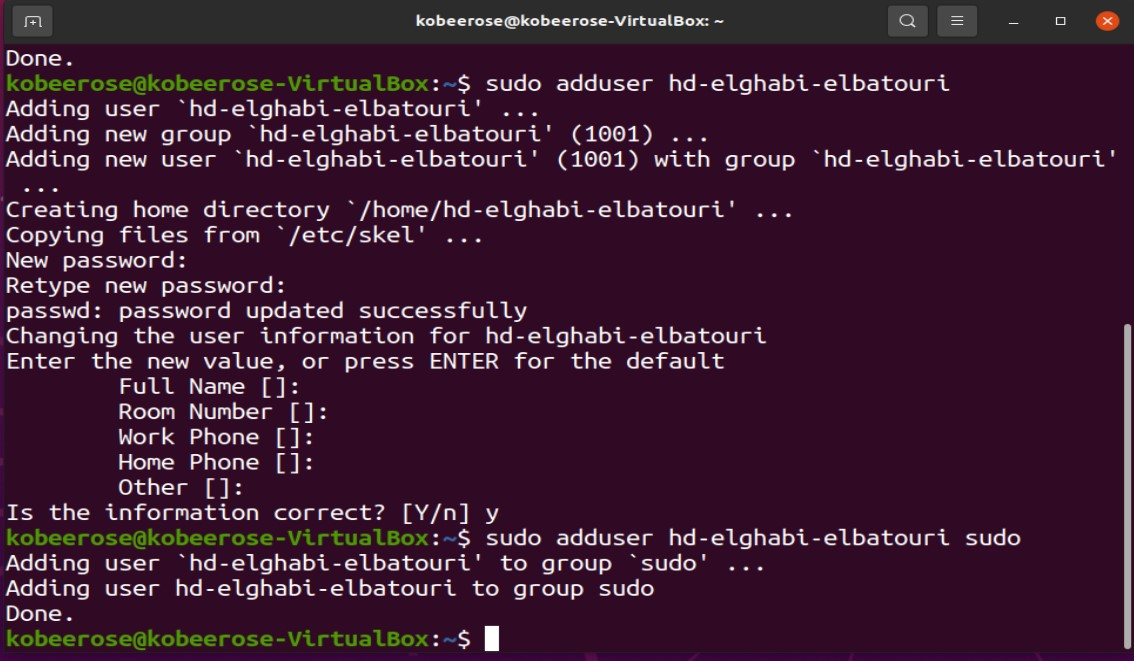
\includegraphics[width=1\linewidth]{Big_Data/Hadoop/Apache Hadoop Installation/Adding new user to sudo group}
\end{center} 
\caption{Adding new user to sudo group} 
\end{figure} 
\FloatBarrier



\par Downloadning Hadoop, Java Development Kit, code_java.zip ( the java source code of the MapReduce "word count" program ), "classpath" script used to set up the variables of the compilation environment, and finally The poeme.txt file to used for manipulations.
\\
\begin{figure}[!htb] 
\begin{center} 
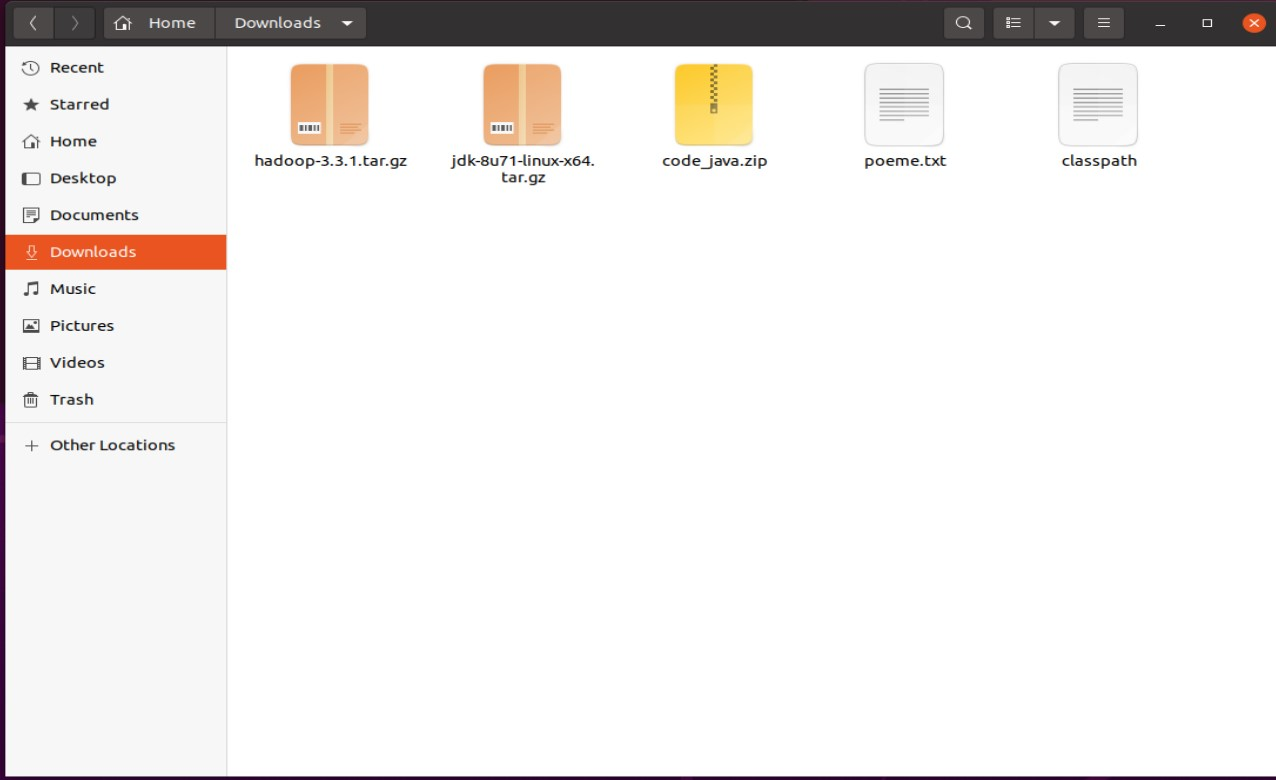
\includegraphics[width=1\linewidth]{Big_Data/Hadoop/Apache Hadoop Installation/Downloading required files} 
\end{center} 
\caption{Downloading required files} 
\end{figure} 
\FloatBarrier

\section{Setting up the ssh key }

\par Install the necessary "openssh-server" package for ssh.
\\
\begin{figure}[!htb] 
\begin{center} 
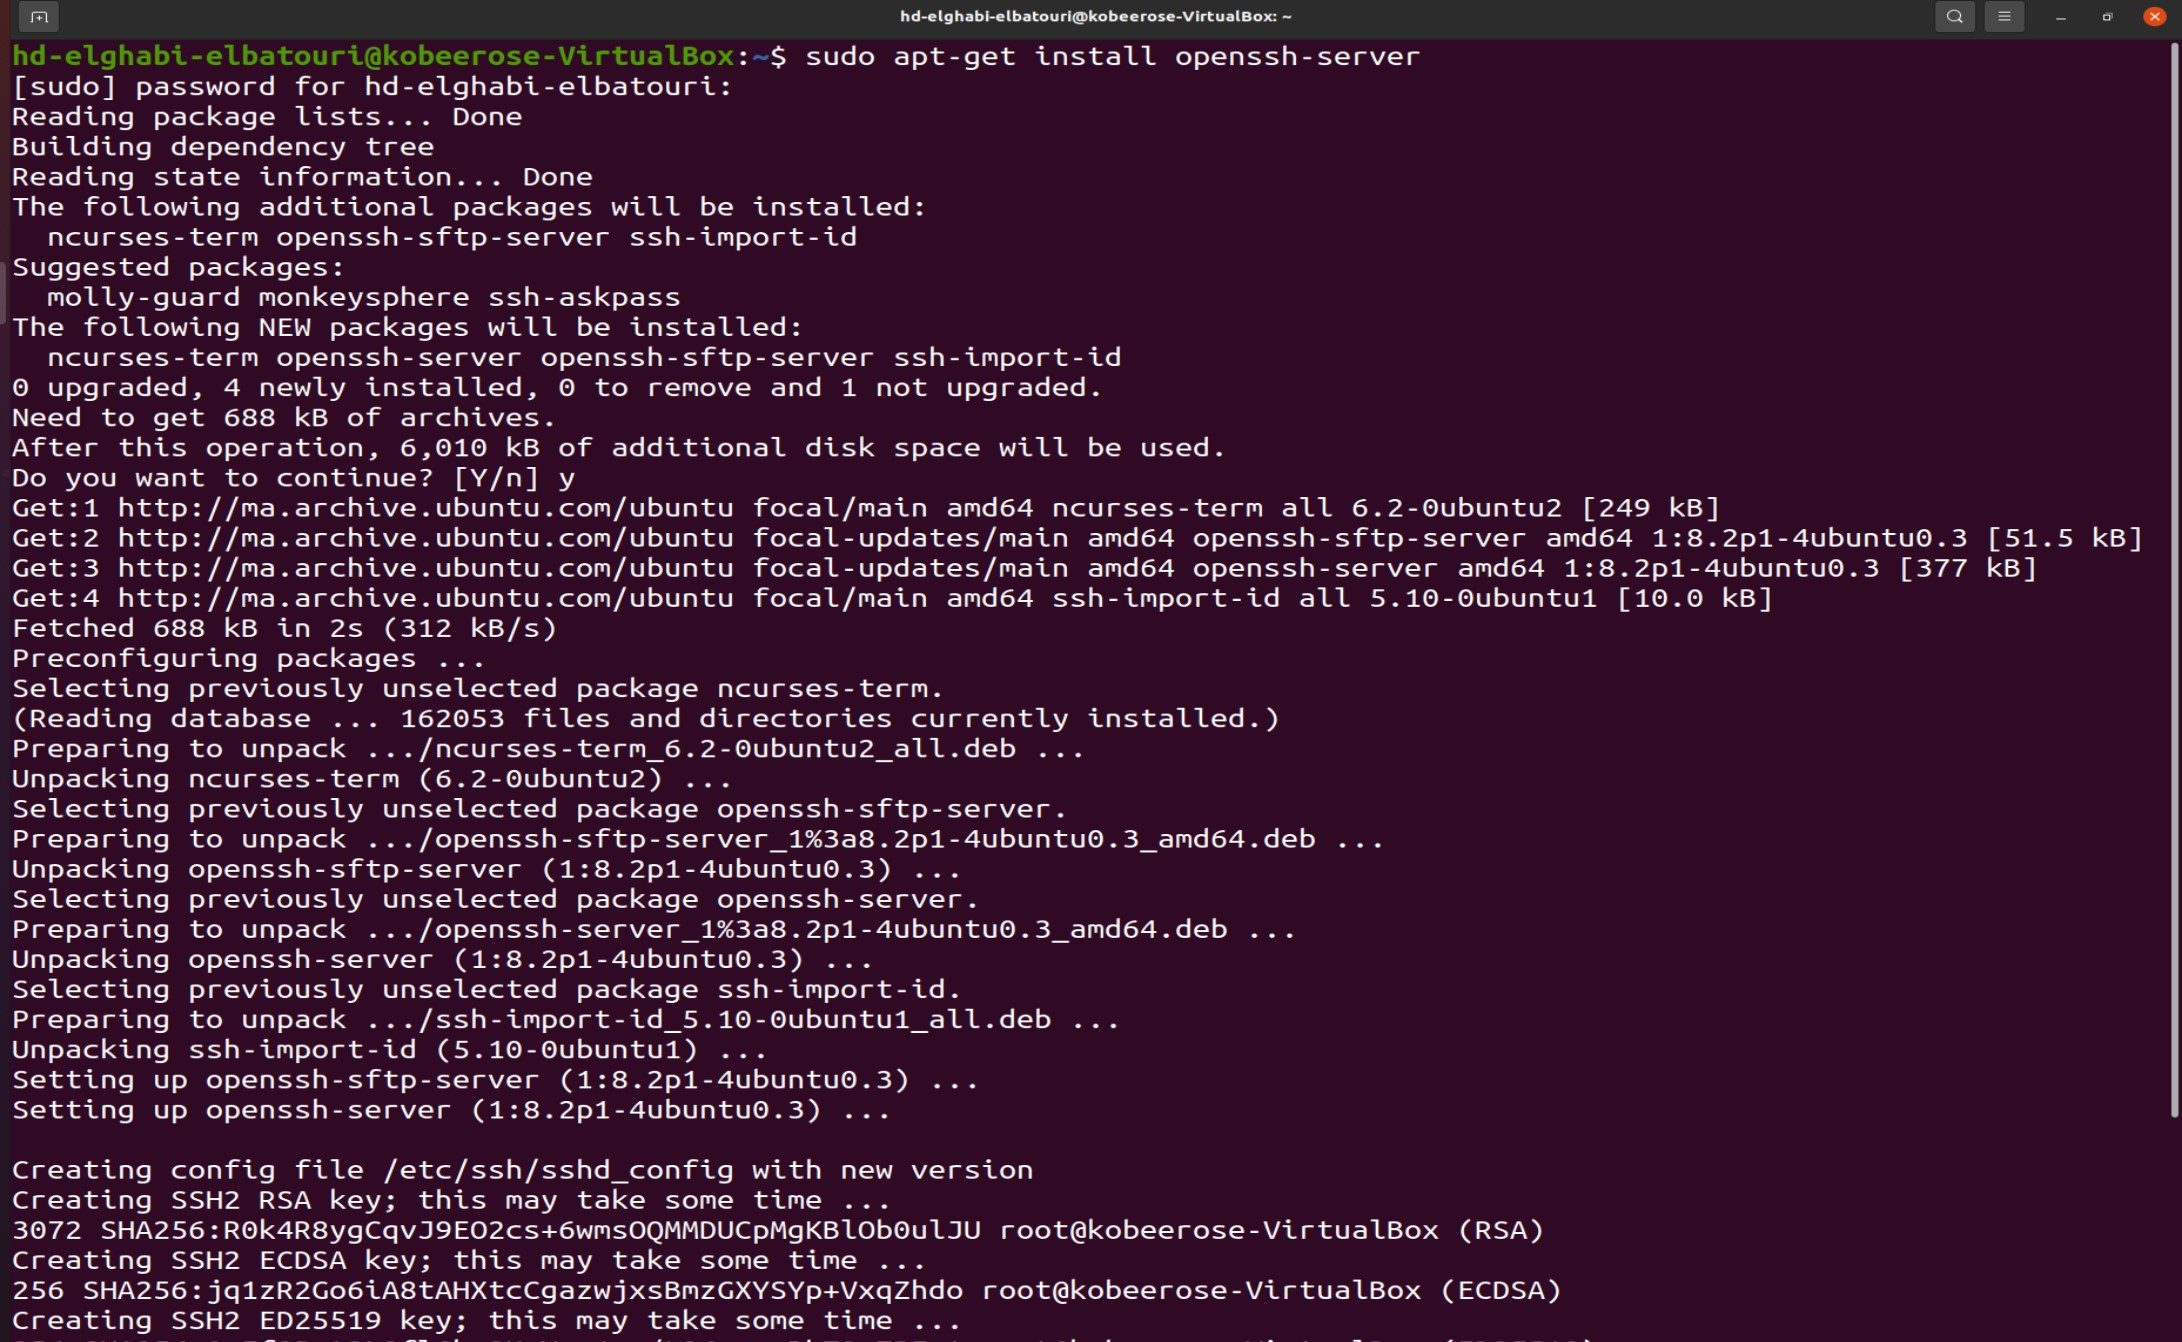
\includegraphics[width=1\linewidth]{Big_Data/Hadoop/Apache Hadoop Installation/Installing openssh-server} 
\end{center} 
\caption{Installing openssh-server} 
\end{figure} 
\FloatBarrier



\par Now you have to set up the ssh key for your own account.
\\
\begin{figure}[!htb] 
\begin{center} 
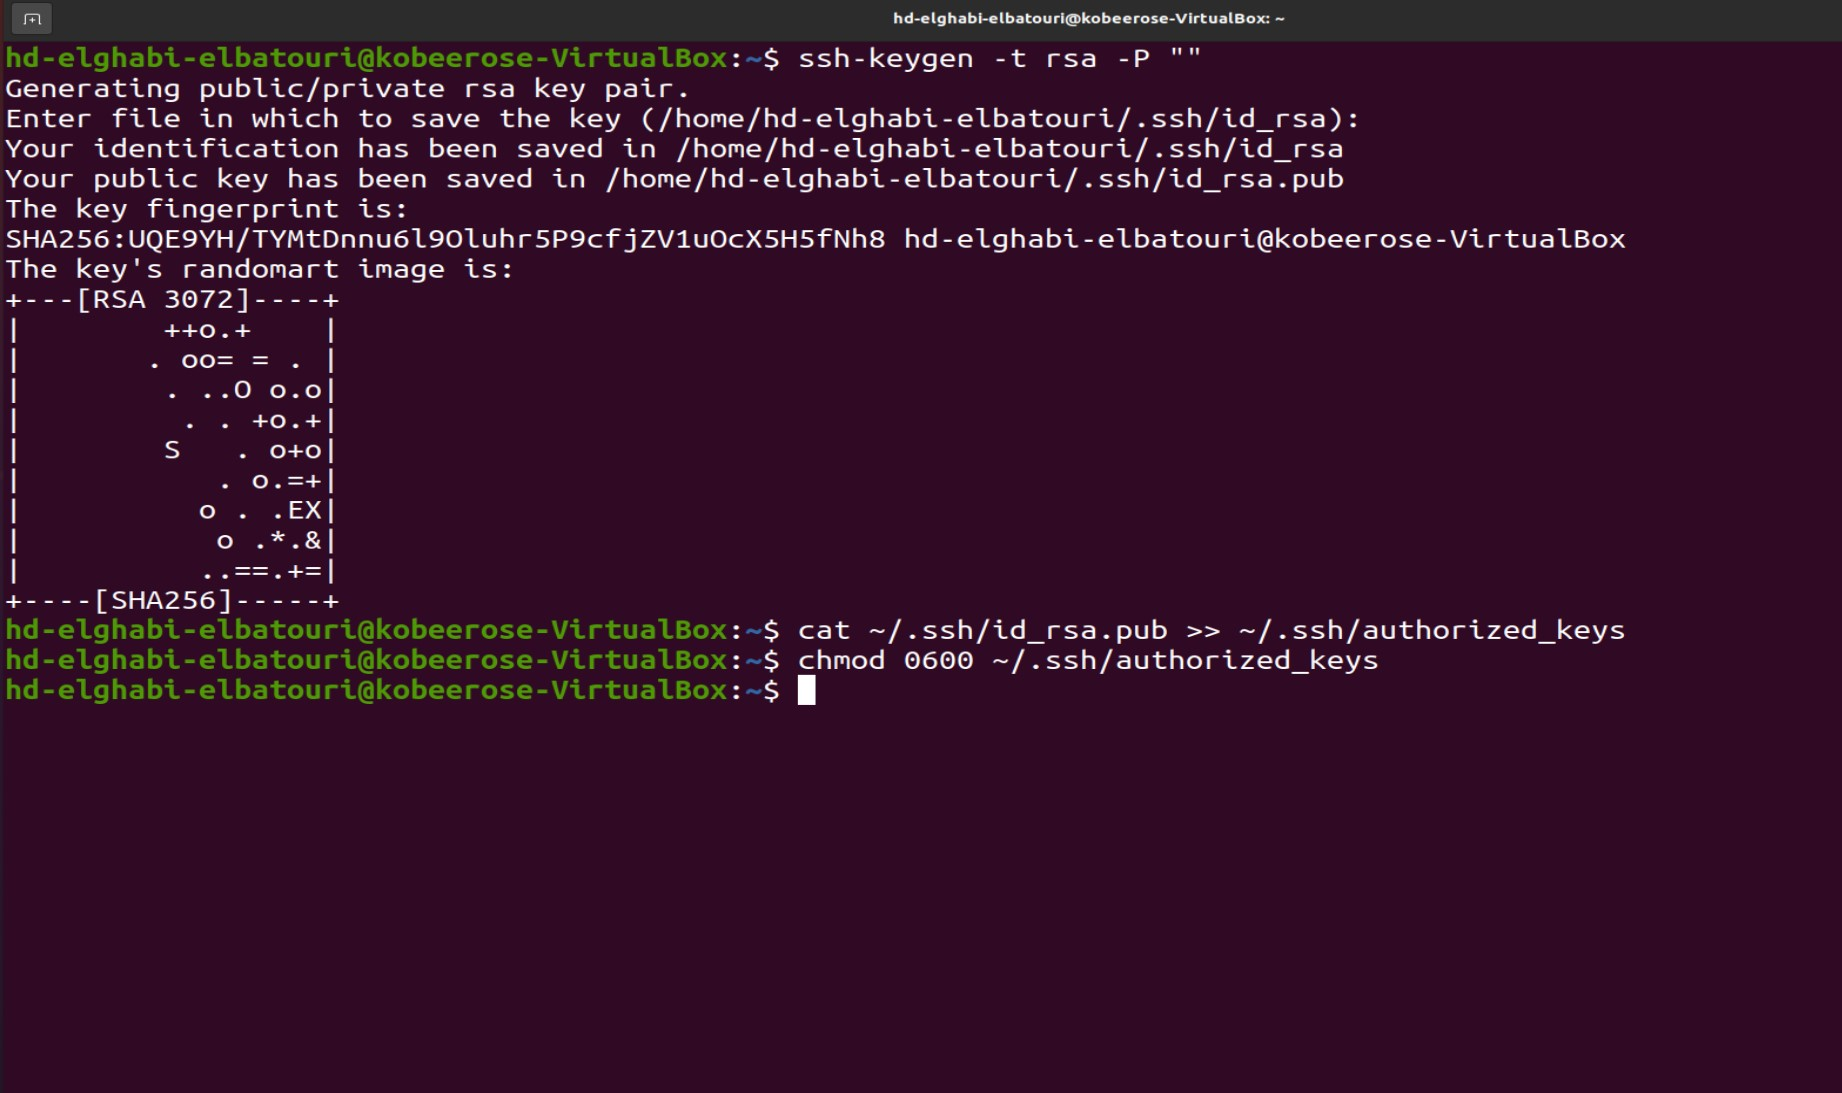
\includegraphics[width=1\linewidth]{Big_Data/Hadoop/Apache Hadoop Installation/Creating SSH key} 
\end{center} 
\caption{Creating SSH key} 
\end{figure} 
\FloatBarrier

\section{Section_name}

\par we Copy the public key to the localhost server.
\\
\begin{figure}[!htb] 
\begin{center} 
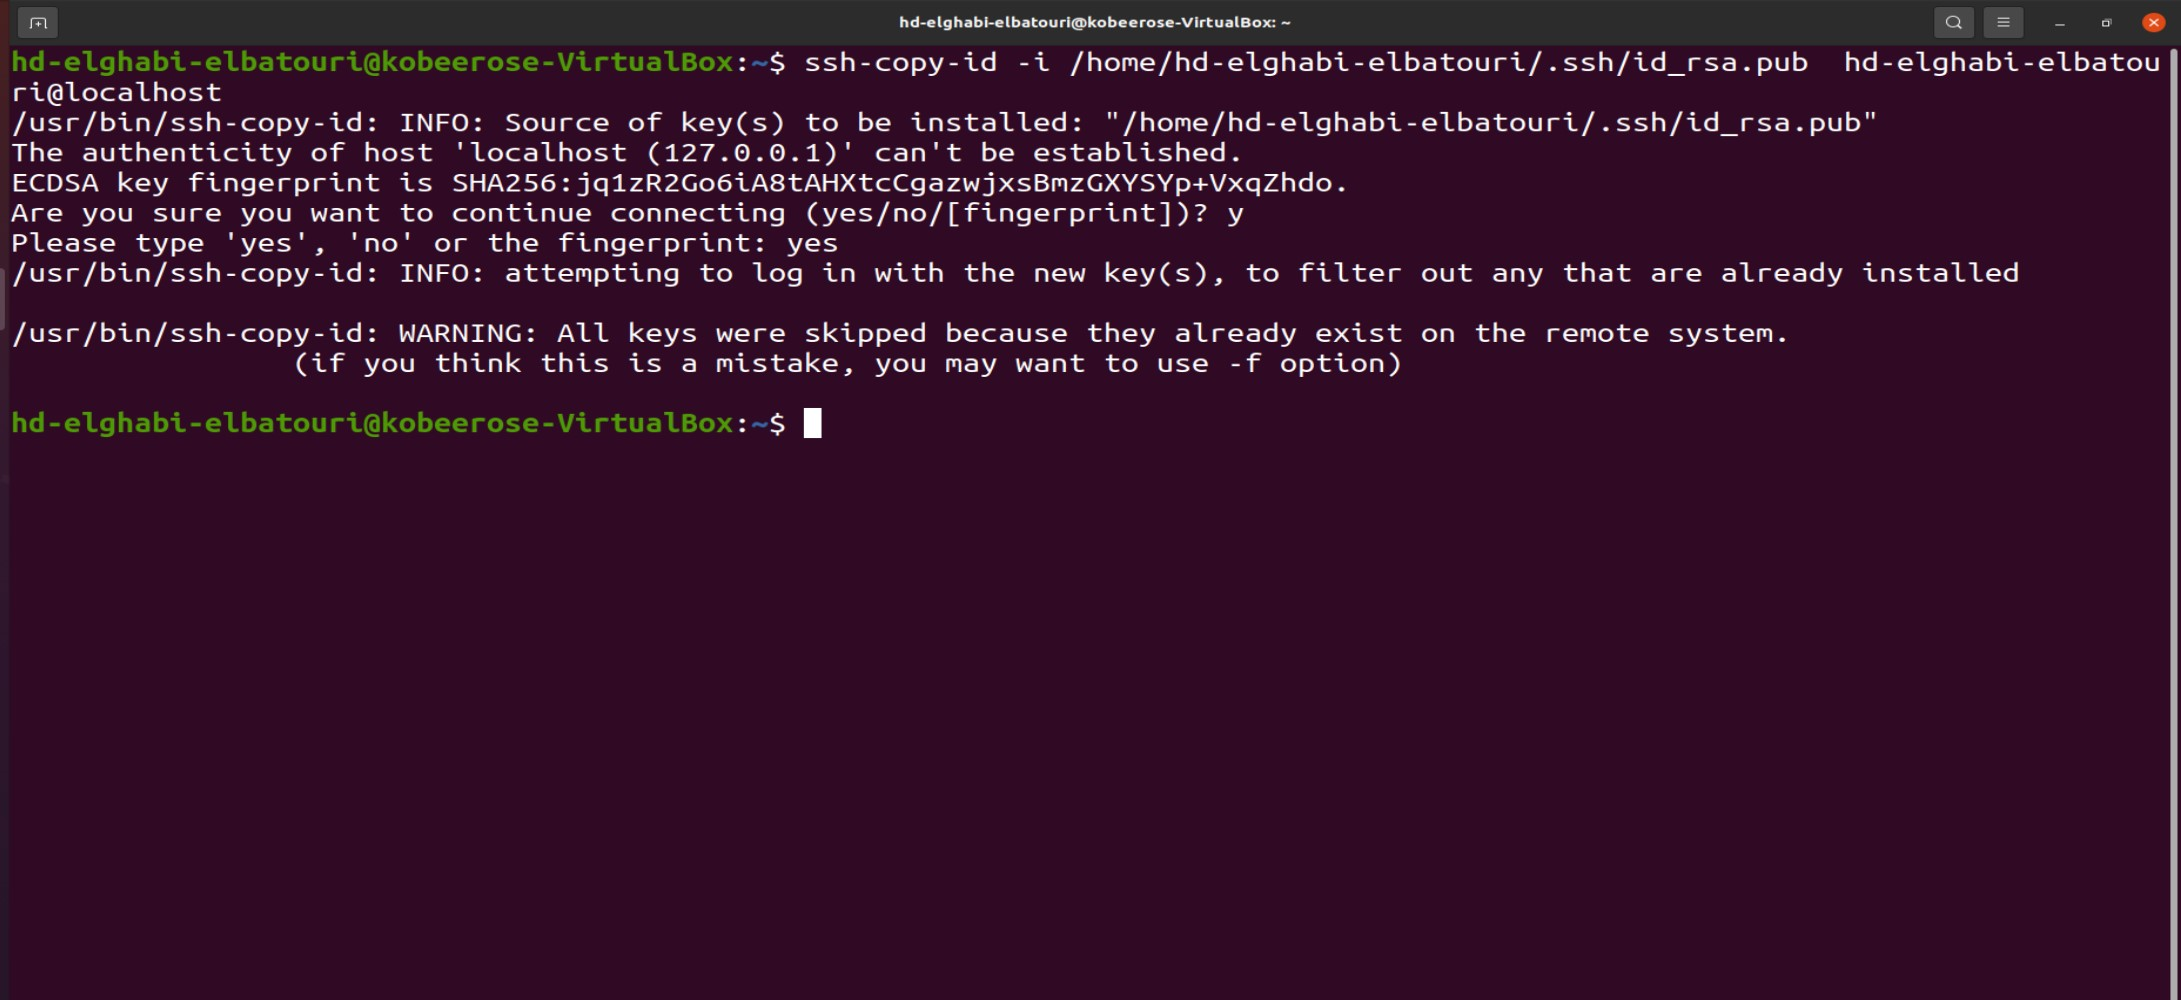
\includegraphics[width=1\linewidth]{Big_Data/Hadoop/Apache Hadoop Installation/Copying the key} 
\end{center} 
\caption{Copying the key} 
\end{figure} 
\FloatBarrier



\par Let's test the connection to localhost.
\\
\begin{figure}[!htb] 
\begin{center} 
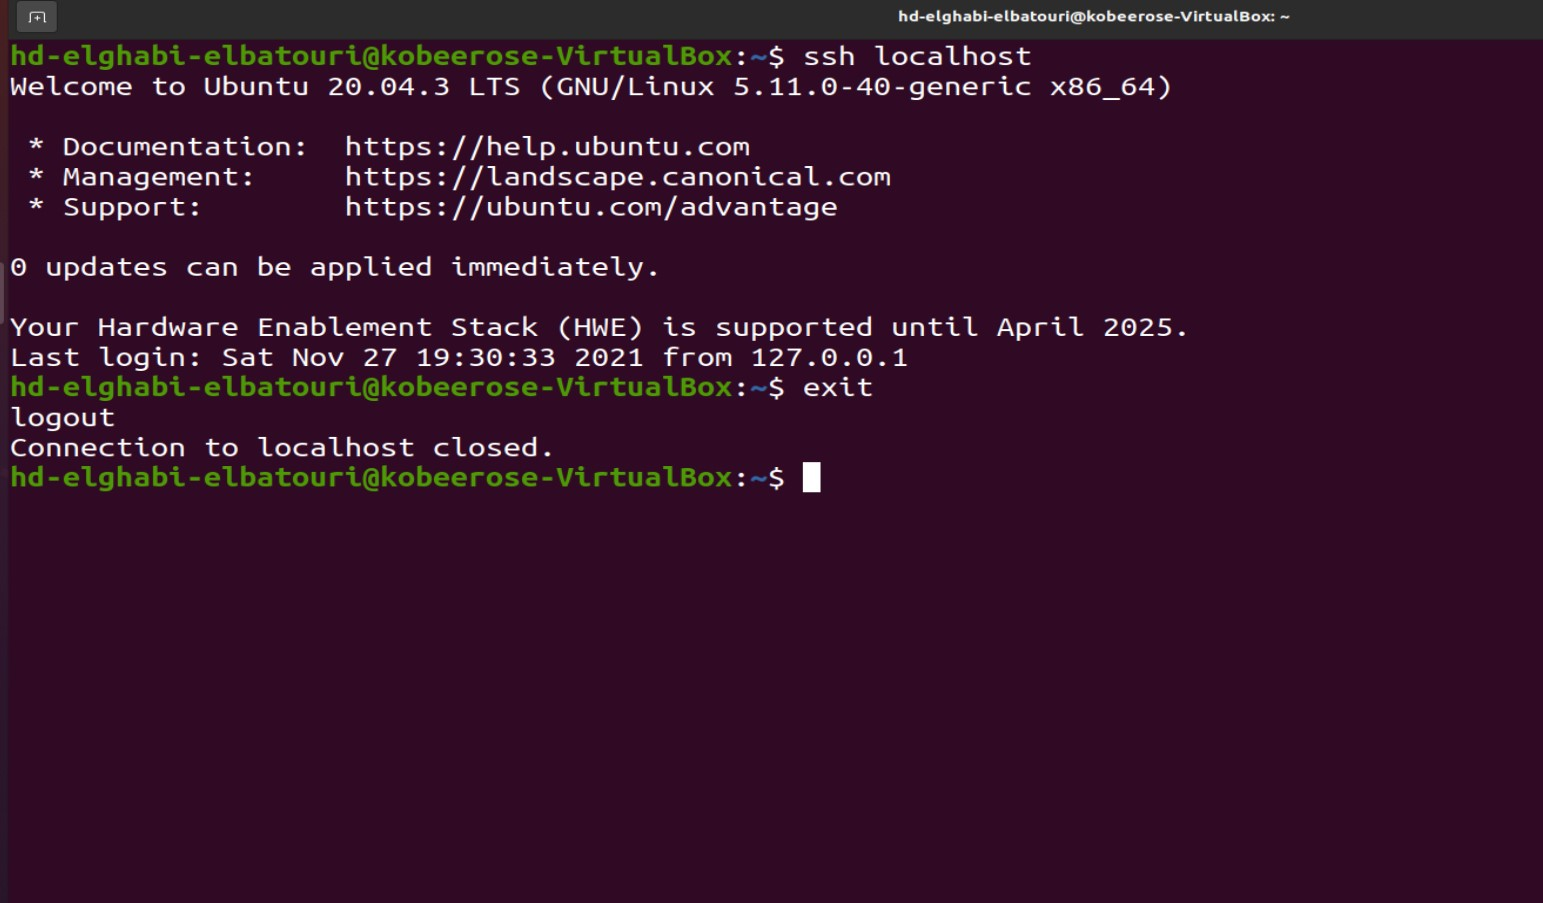
\includegraphics[width=1\linewidth]{Big_Data/Hadoop/Apache Hadoop Installation/Connecting to localhost} 
\end{center} 
\caption{Connecting to localhost} 
\end{figure} 
\FloatBarrier

\section{Installing JAVA 8}

\par We will install in the / opt / java directory to ensure a global access.
\\
\begin{figure}[!htb] 
\begin{center} 
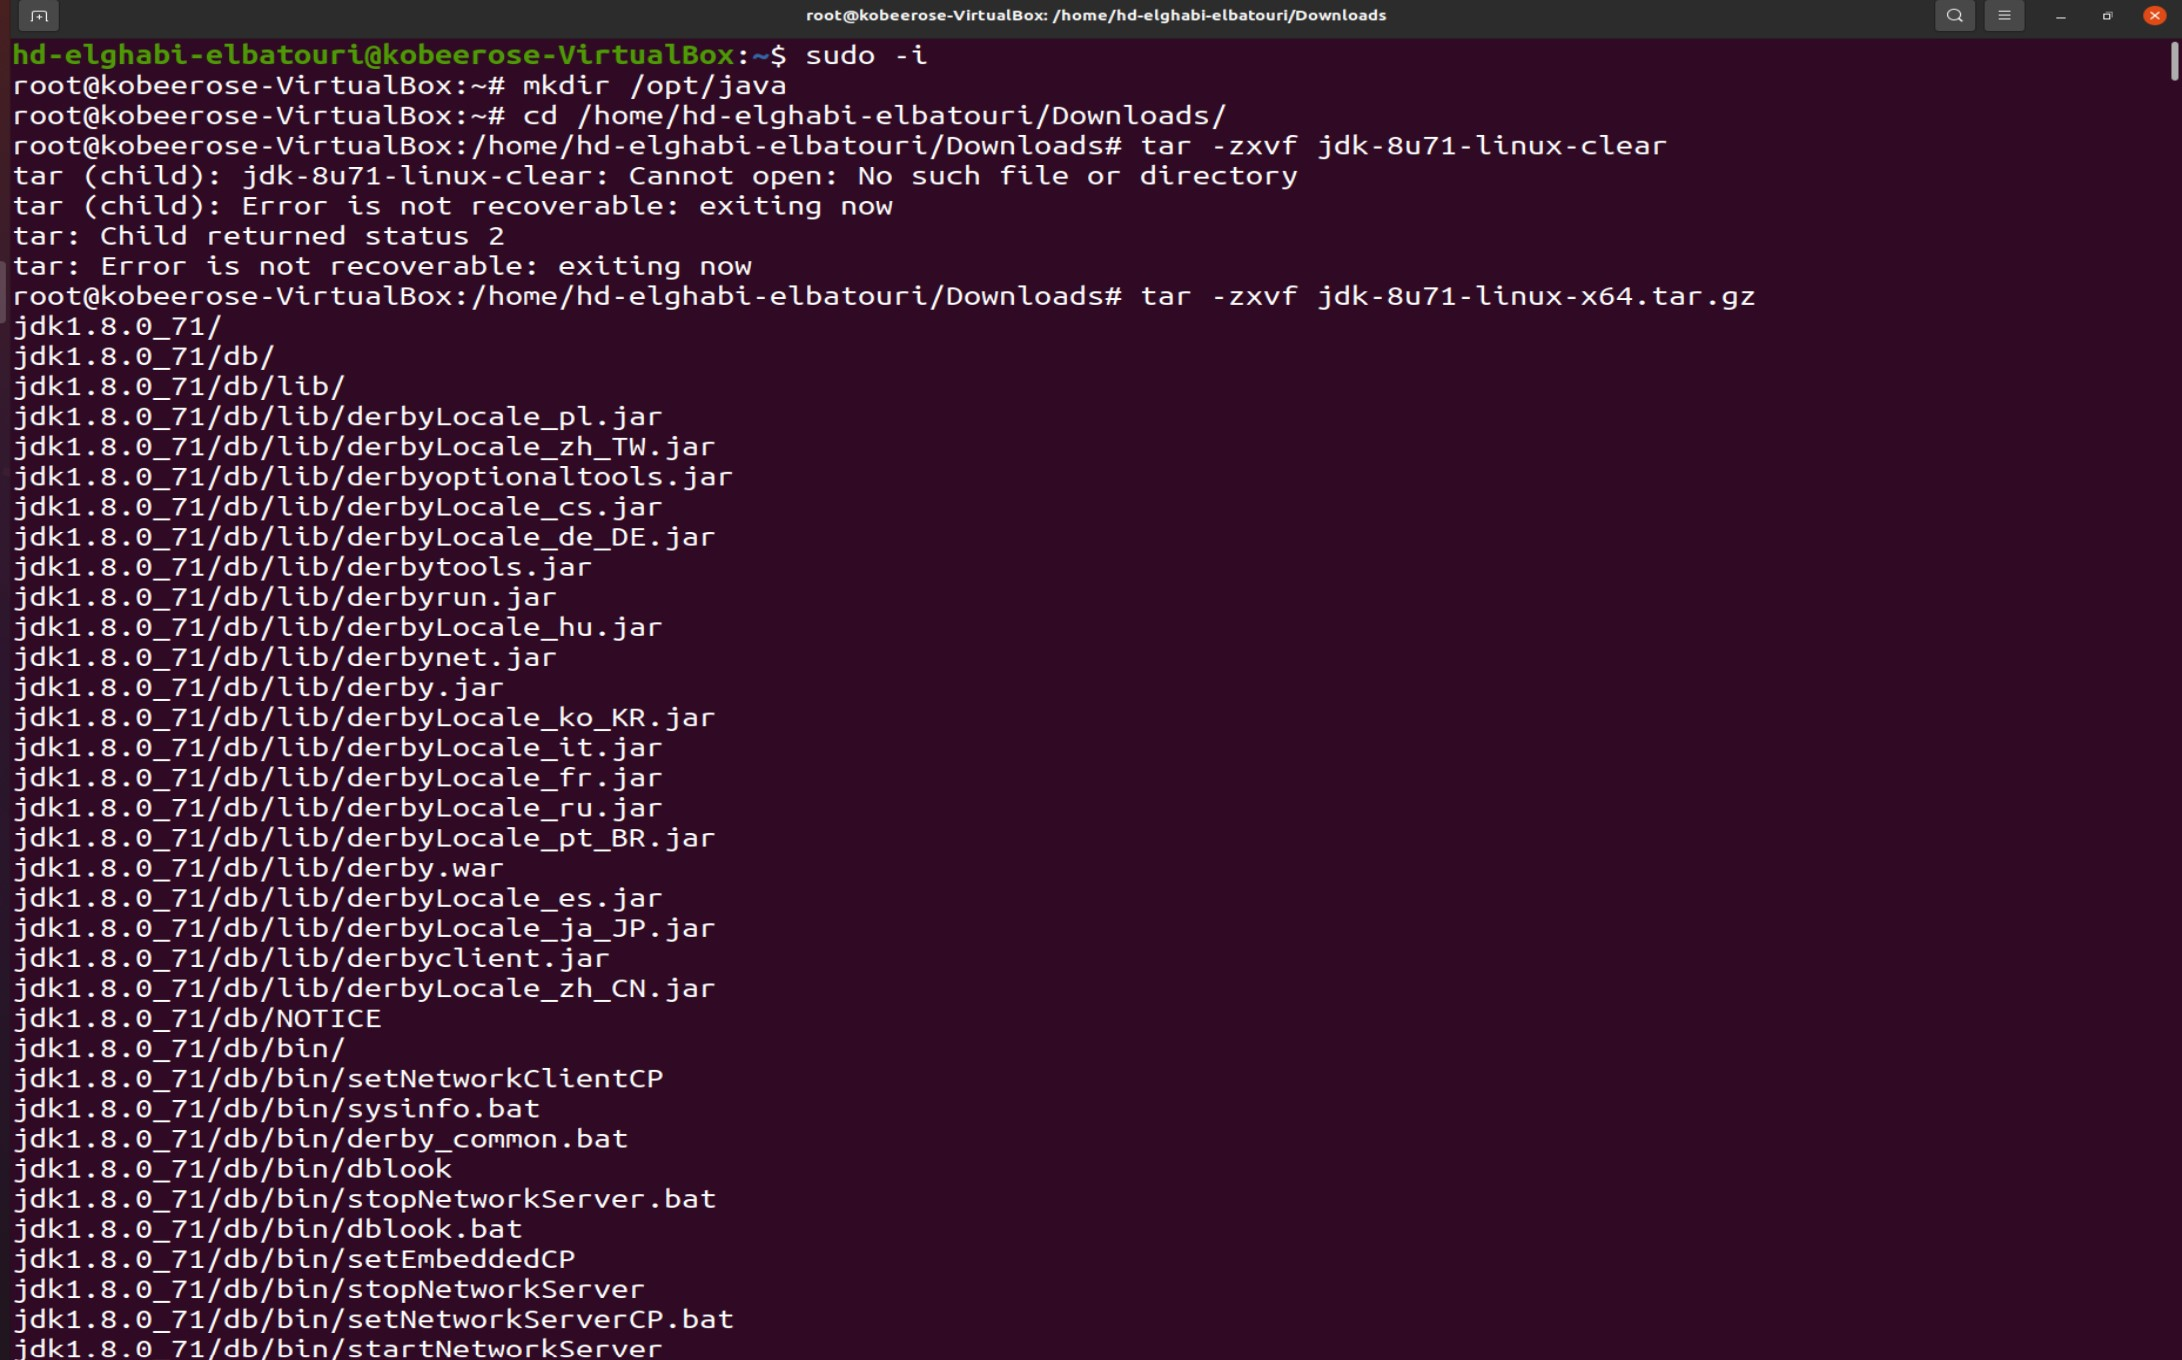
\includegraphics[width=1\linewidth]{Big_Data/Hadoop/Apache Hadoop Installation/Extracting files} 
\end{center} 
\caption{Extracting files} 
\end{figure} 
\FloatBarrier

\begin{figure}[!htb] 
\begin{center} 
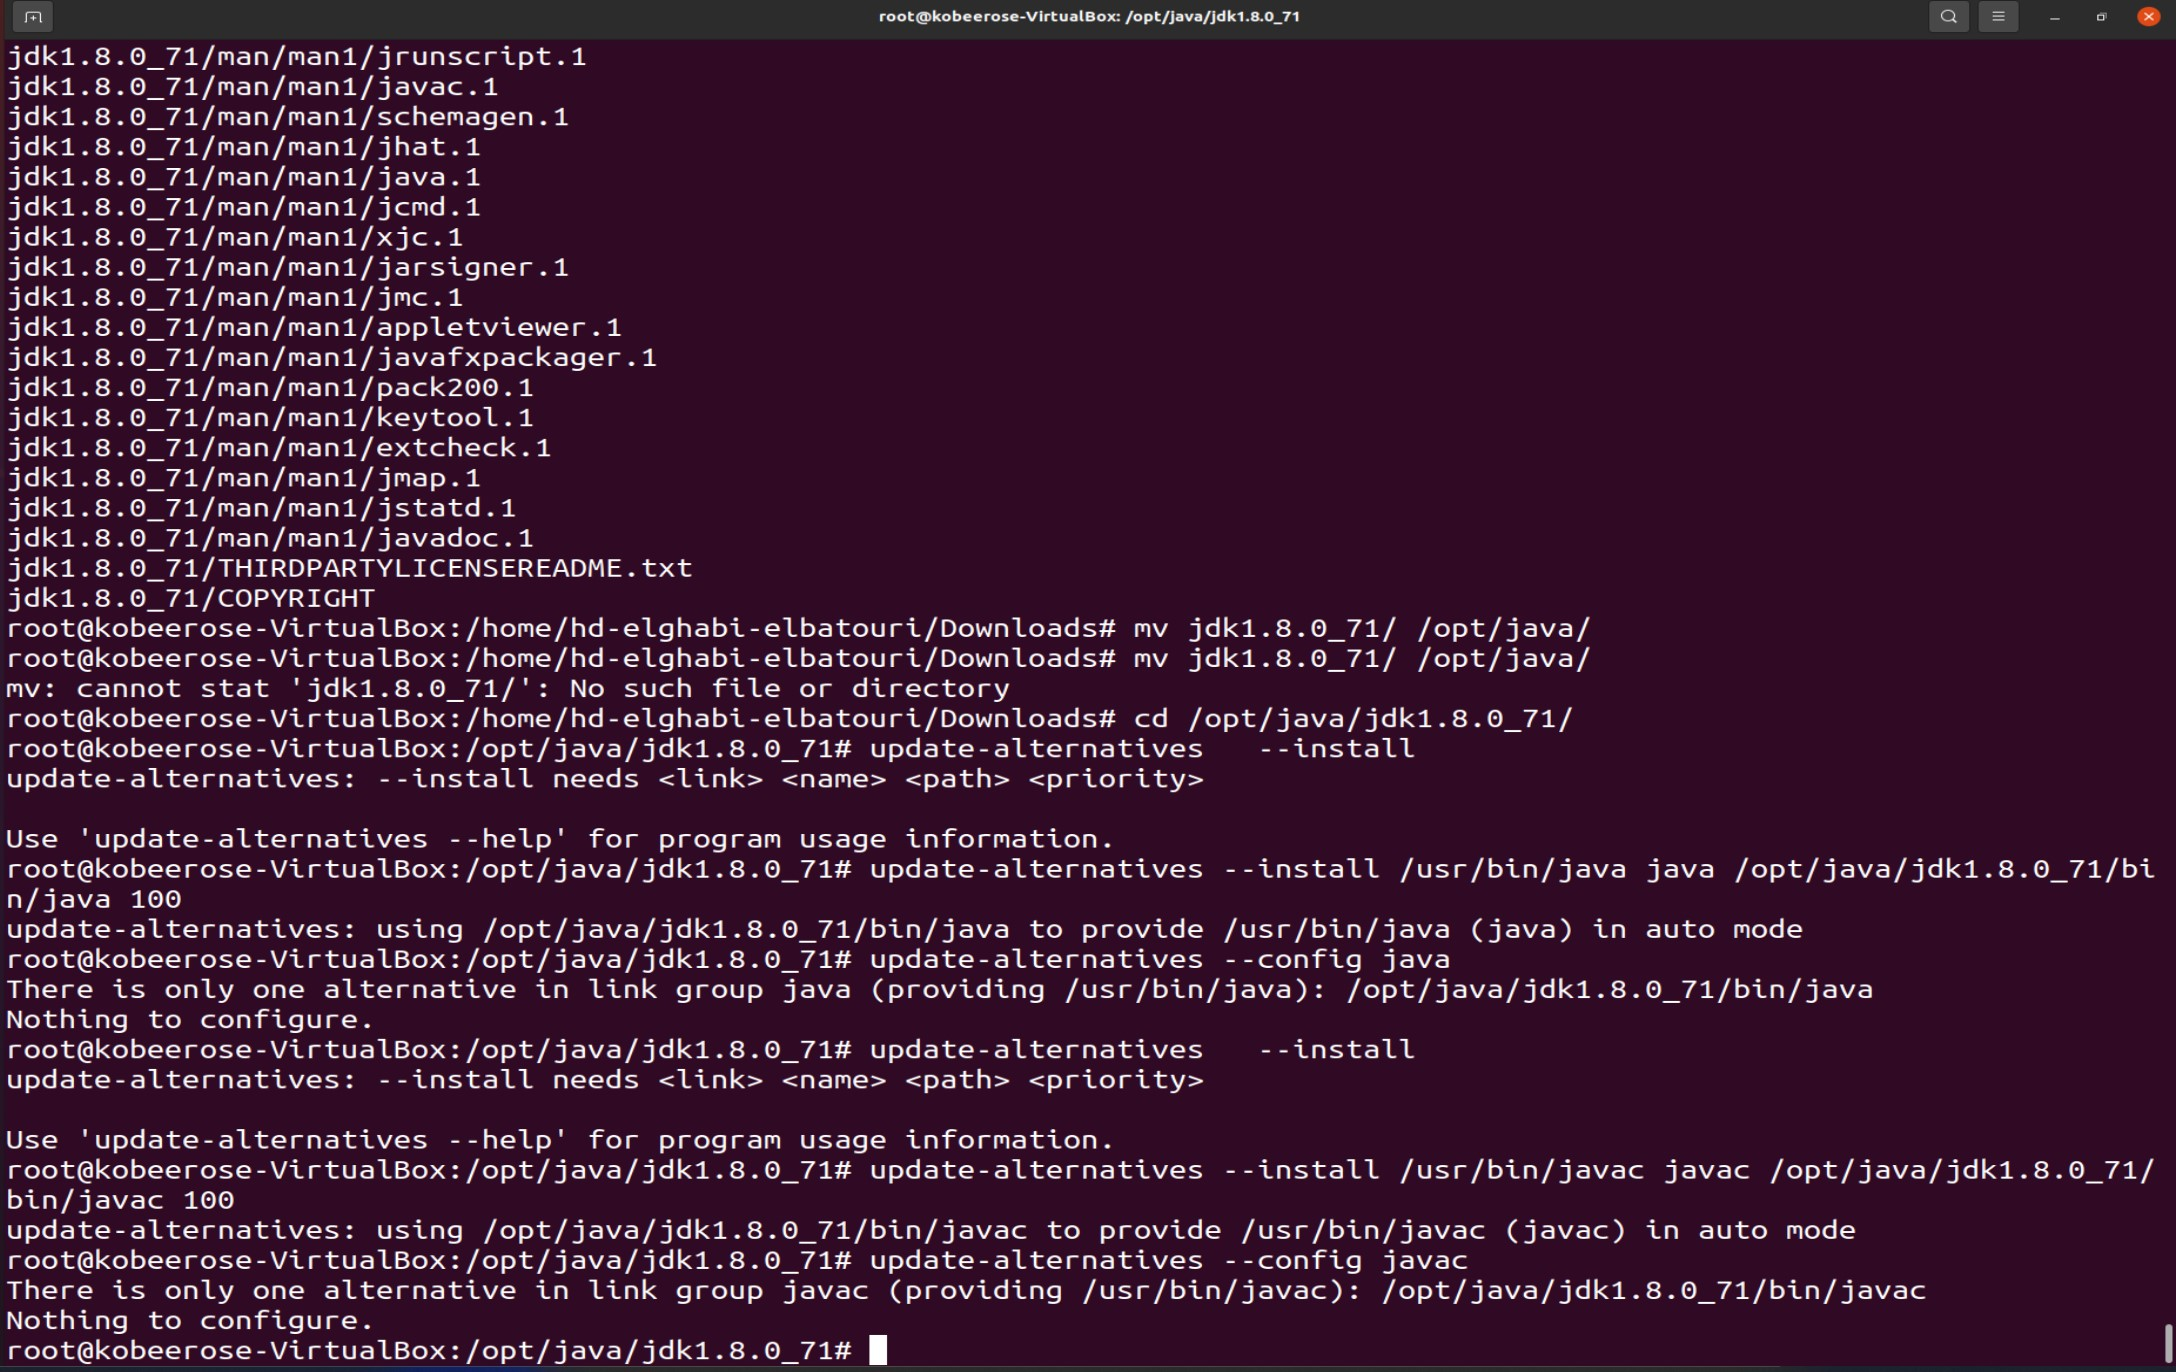
\includegraphics[width=1\linewidth]{Big_Data/Hadoop/Apache Hadoop Installation/Installing java and javac} 
\end{center} 
\caption{Installing java and javac} 
\end{figure} 
\FloatBarrier


\par To permanently set up JAVA environment variables for all users, we will configure profile file.
\\
\begin{figure}[!htb] 
\begin{center} 
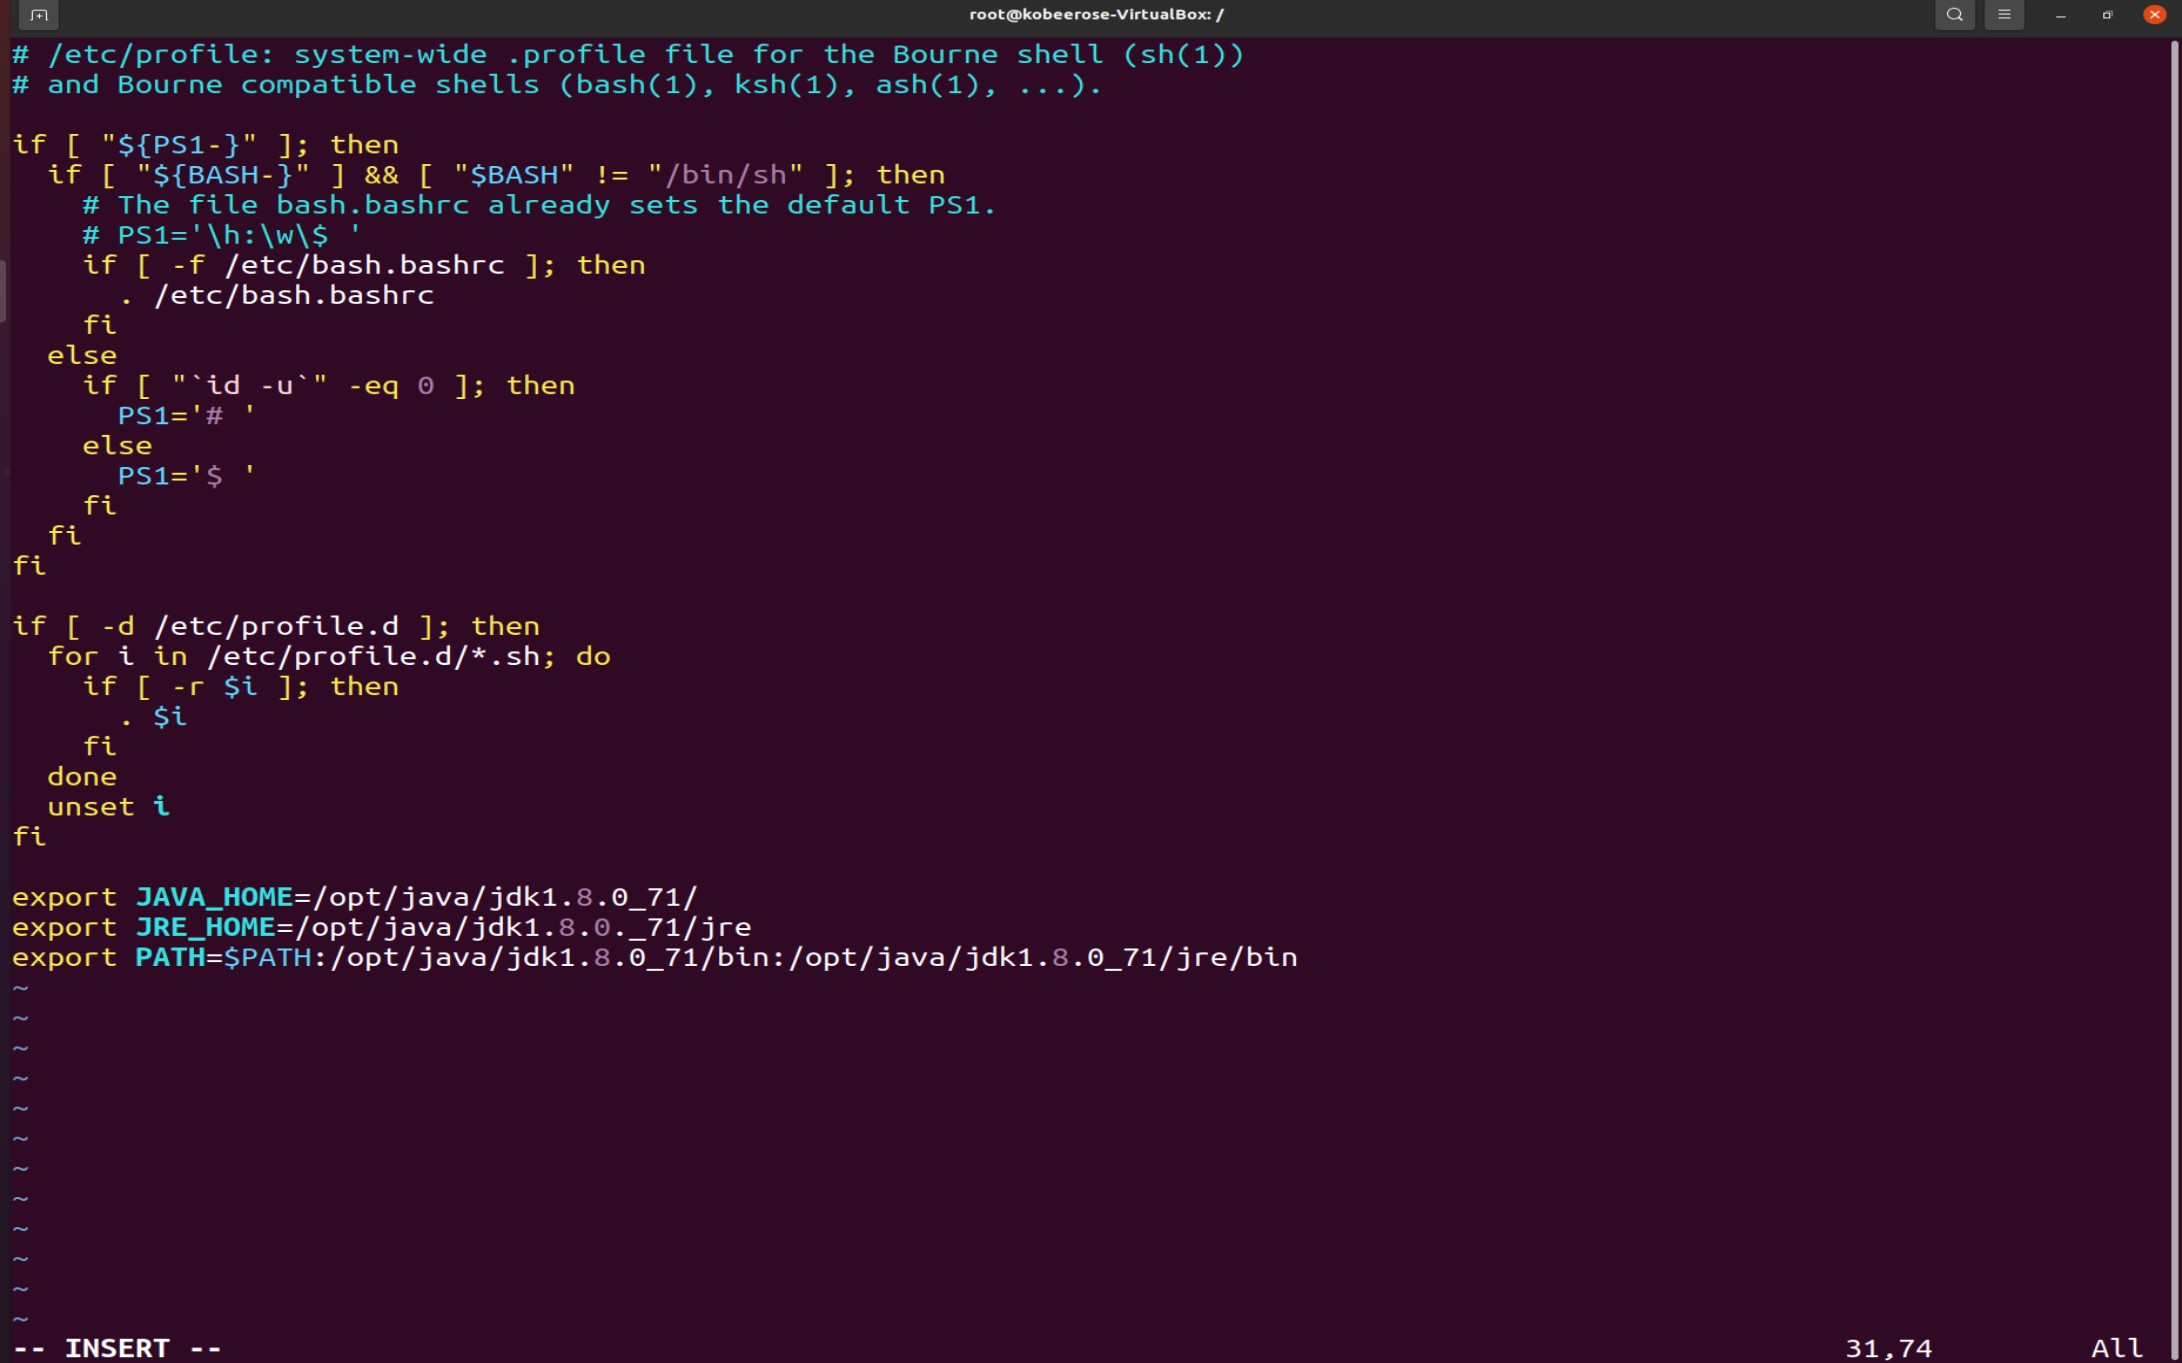
\includegraphics[width=1\linewidth]{Big_Data/Hadoop/Apache Hadoop Installation/profile file config} 
\end{center} 
\caption{profile file config} 
\end{figure} 
\FloatBarrier

\par Le'ts can test the setting of environment variables in the hadoop terminal.
\\
\begin{figure}[!htb] 
\begin{center} 
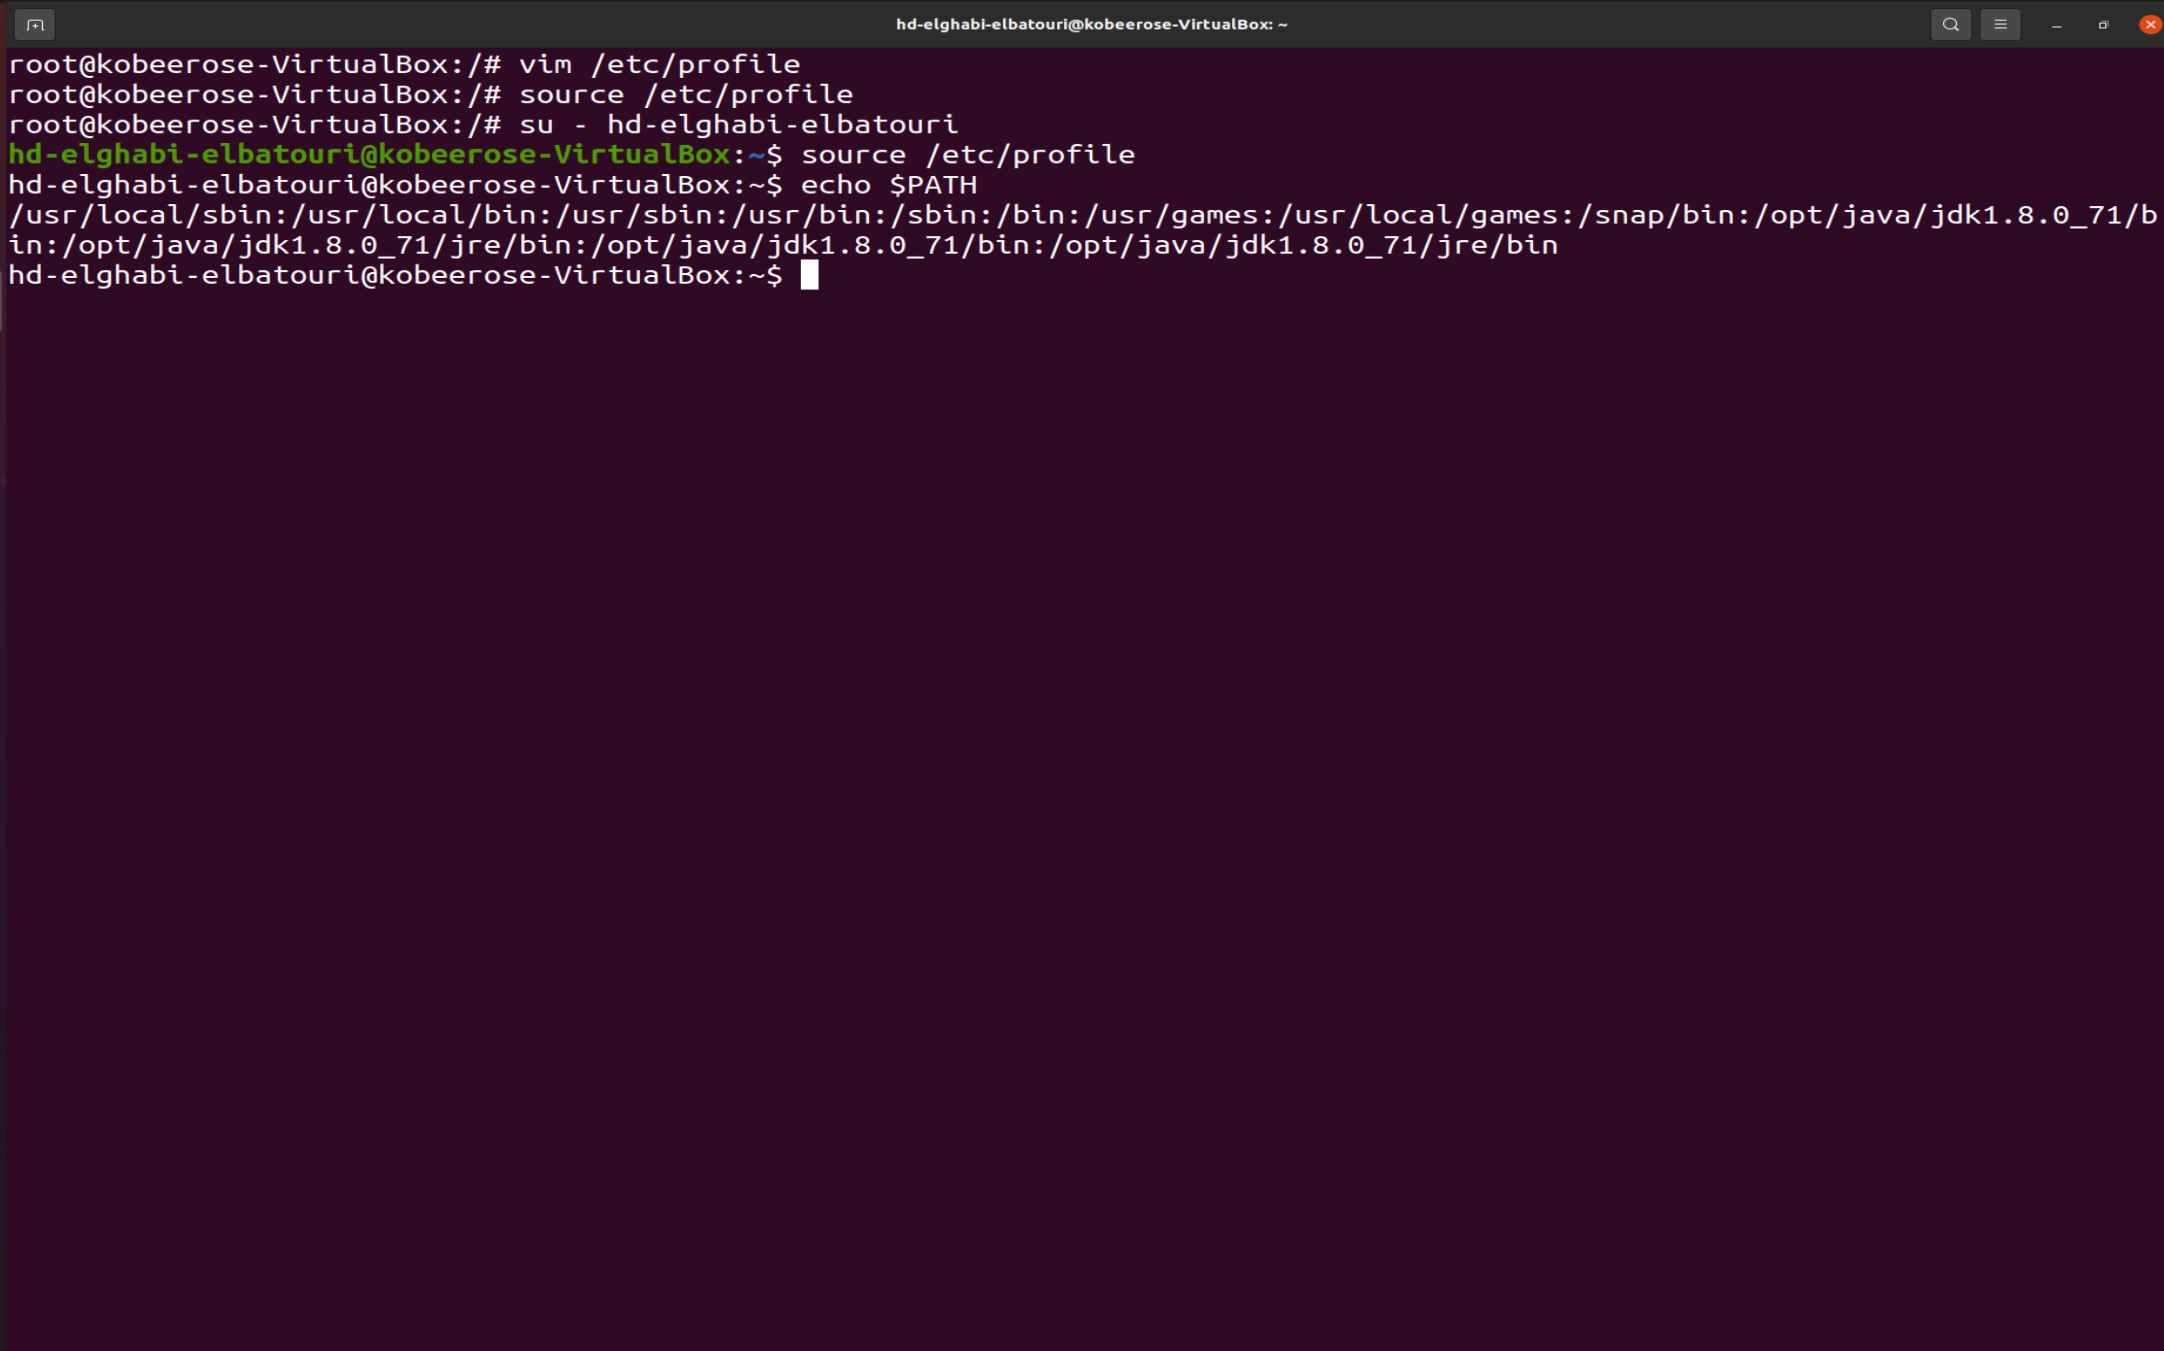
\includegraphics[width=1\linewidth]{Big_Data/Hadoop/Apache Hadoop Installation/Verifying PATH} 
\end{center} 
\caption{Verifying PATH} 
\end{figure} 
\FloatBarrier

\section{Installing Apache Hadoop 3.3.1}

\par Extracting files and Installing Apache Hadoop.
\\
\begin{figure}[!htb] 
\begin{center} 
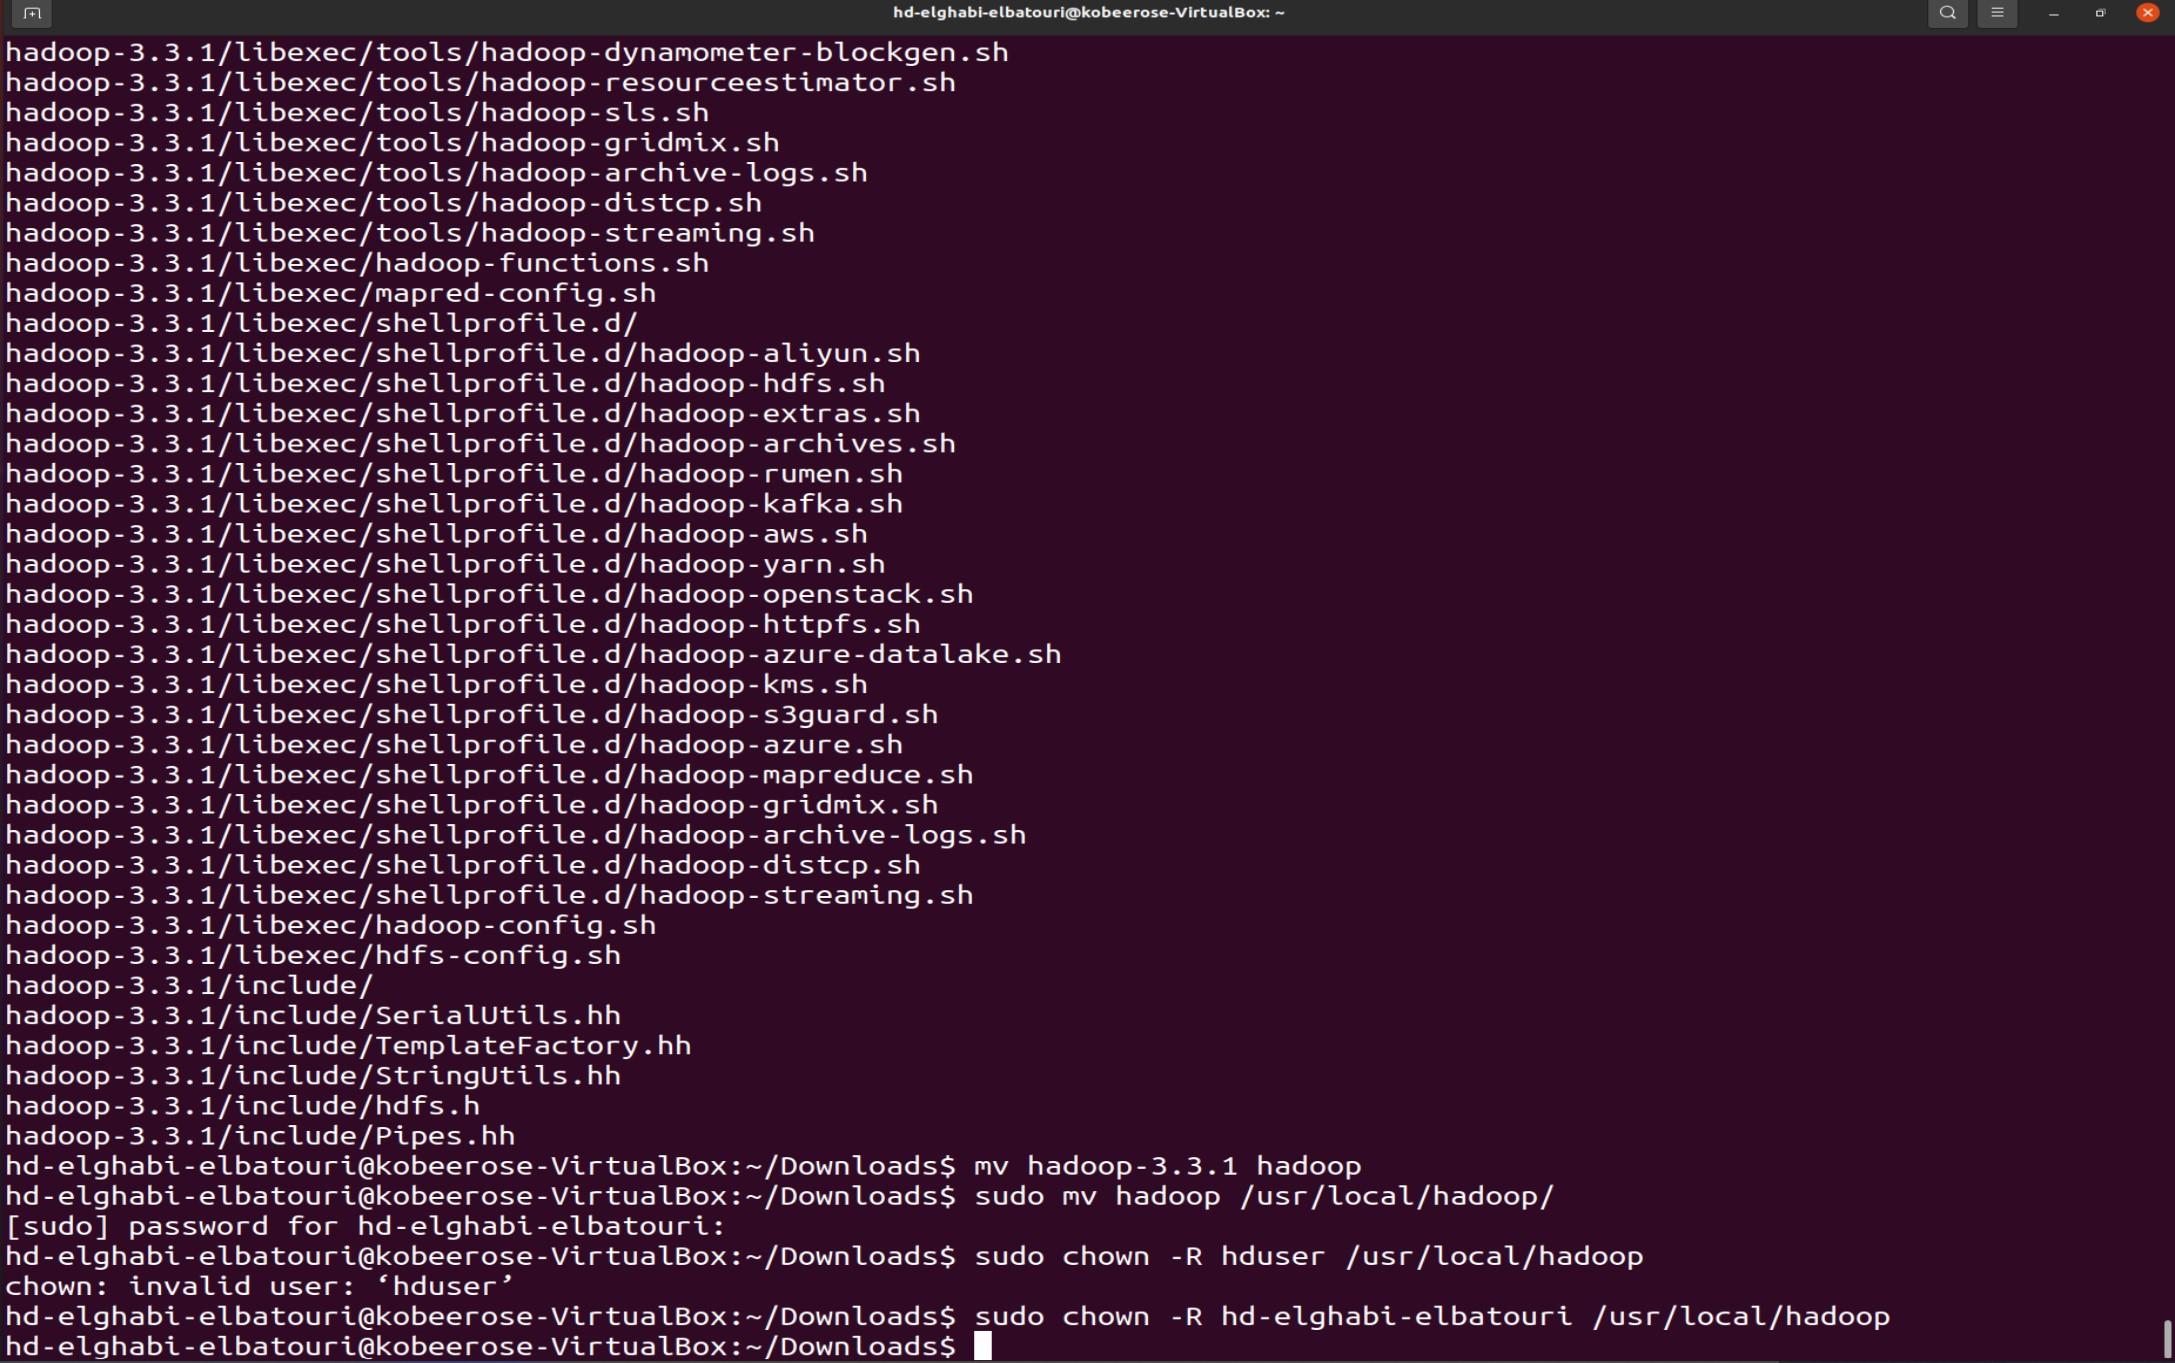
\includegraphics[width=1\linewidth]{Big_Data/Hadoop/Apache Hadoop Installation/Extracting Hadoop}
\end{center} 
\caption{Extracting Hadoop} 
\end{figure} 
\FloatBarrier


\par Create the hadoop data storage directories.
\\
\begin{figure}[!htb] 
\begin{center} 
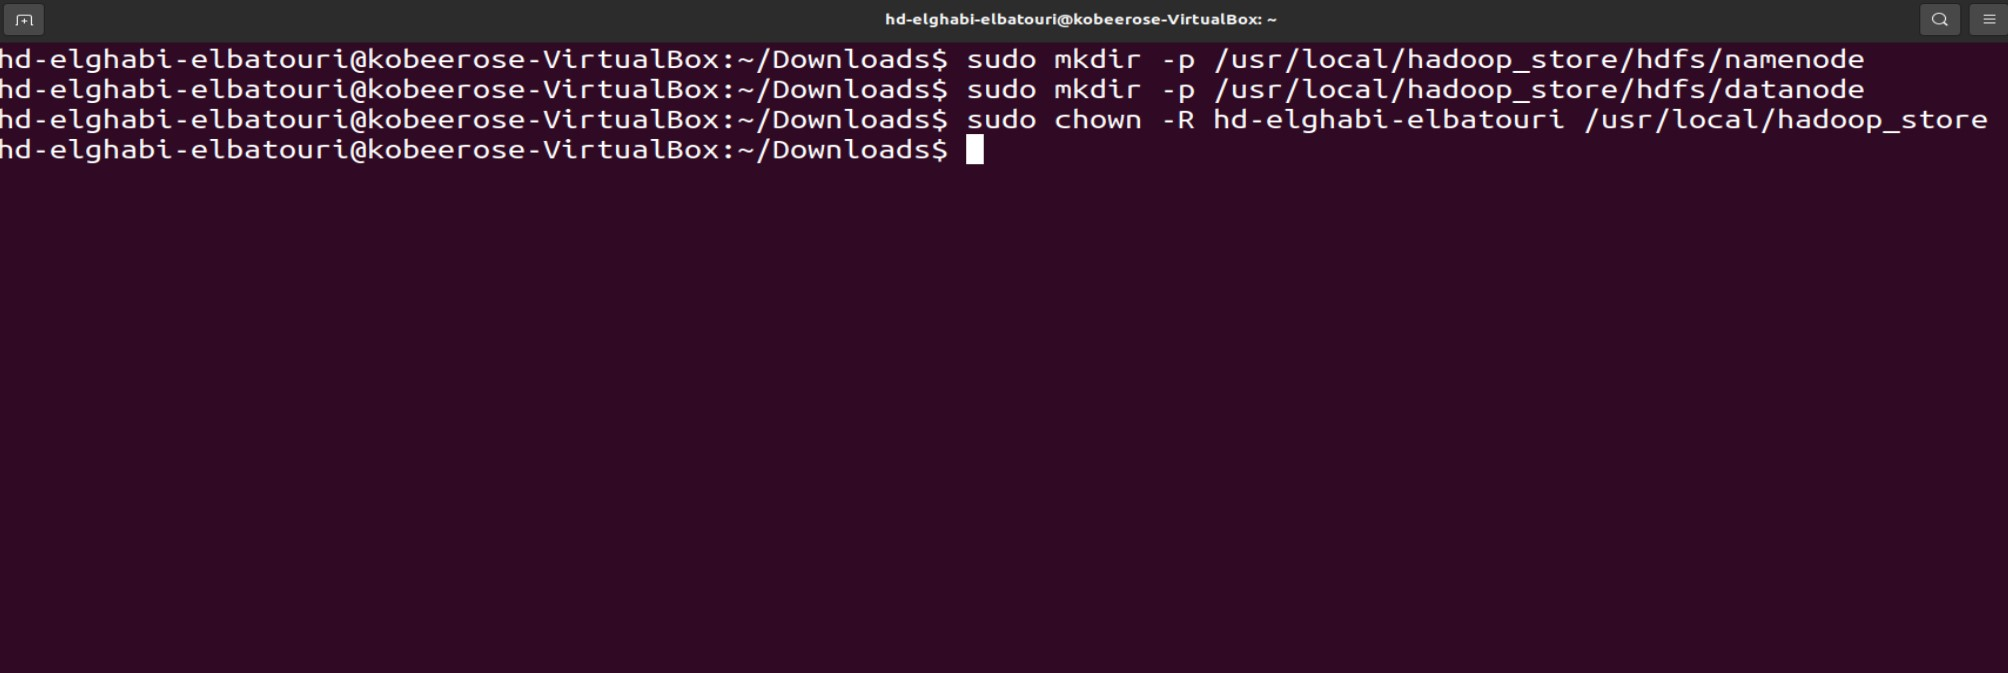
\includegraphics[width=1\linewidth]{Big_Data/Hadoop/Apache Hadoop Installation/Creating Storage repo} 
\end{center} 
\caption{Creating Storage repo} 
\end{figure} 
\FloatBarrier

\section{Configuring Apache Hadoop 3.3.1 }

\par Setting up environment variables for Hadoop.
\\
\begin{figure}[!htb] 
\begin{center} 
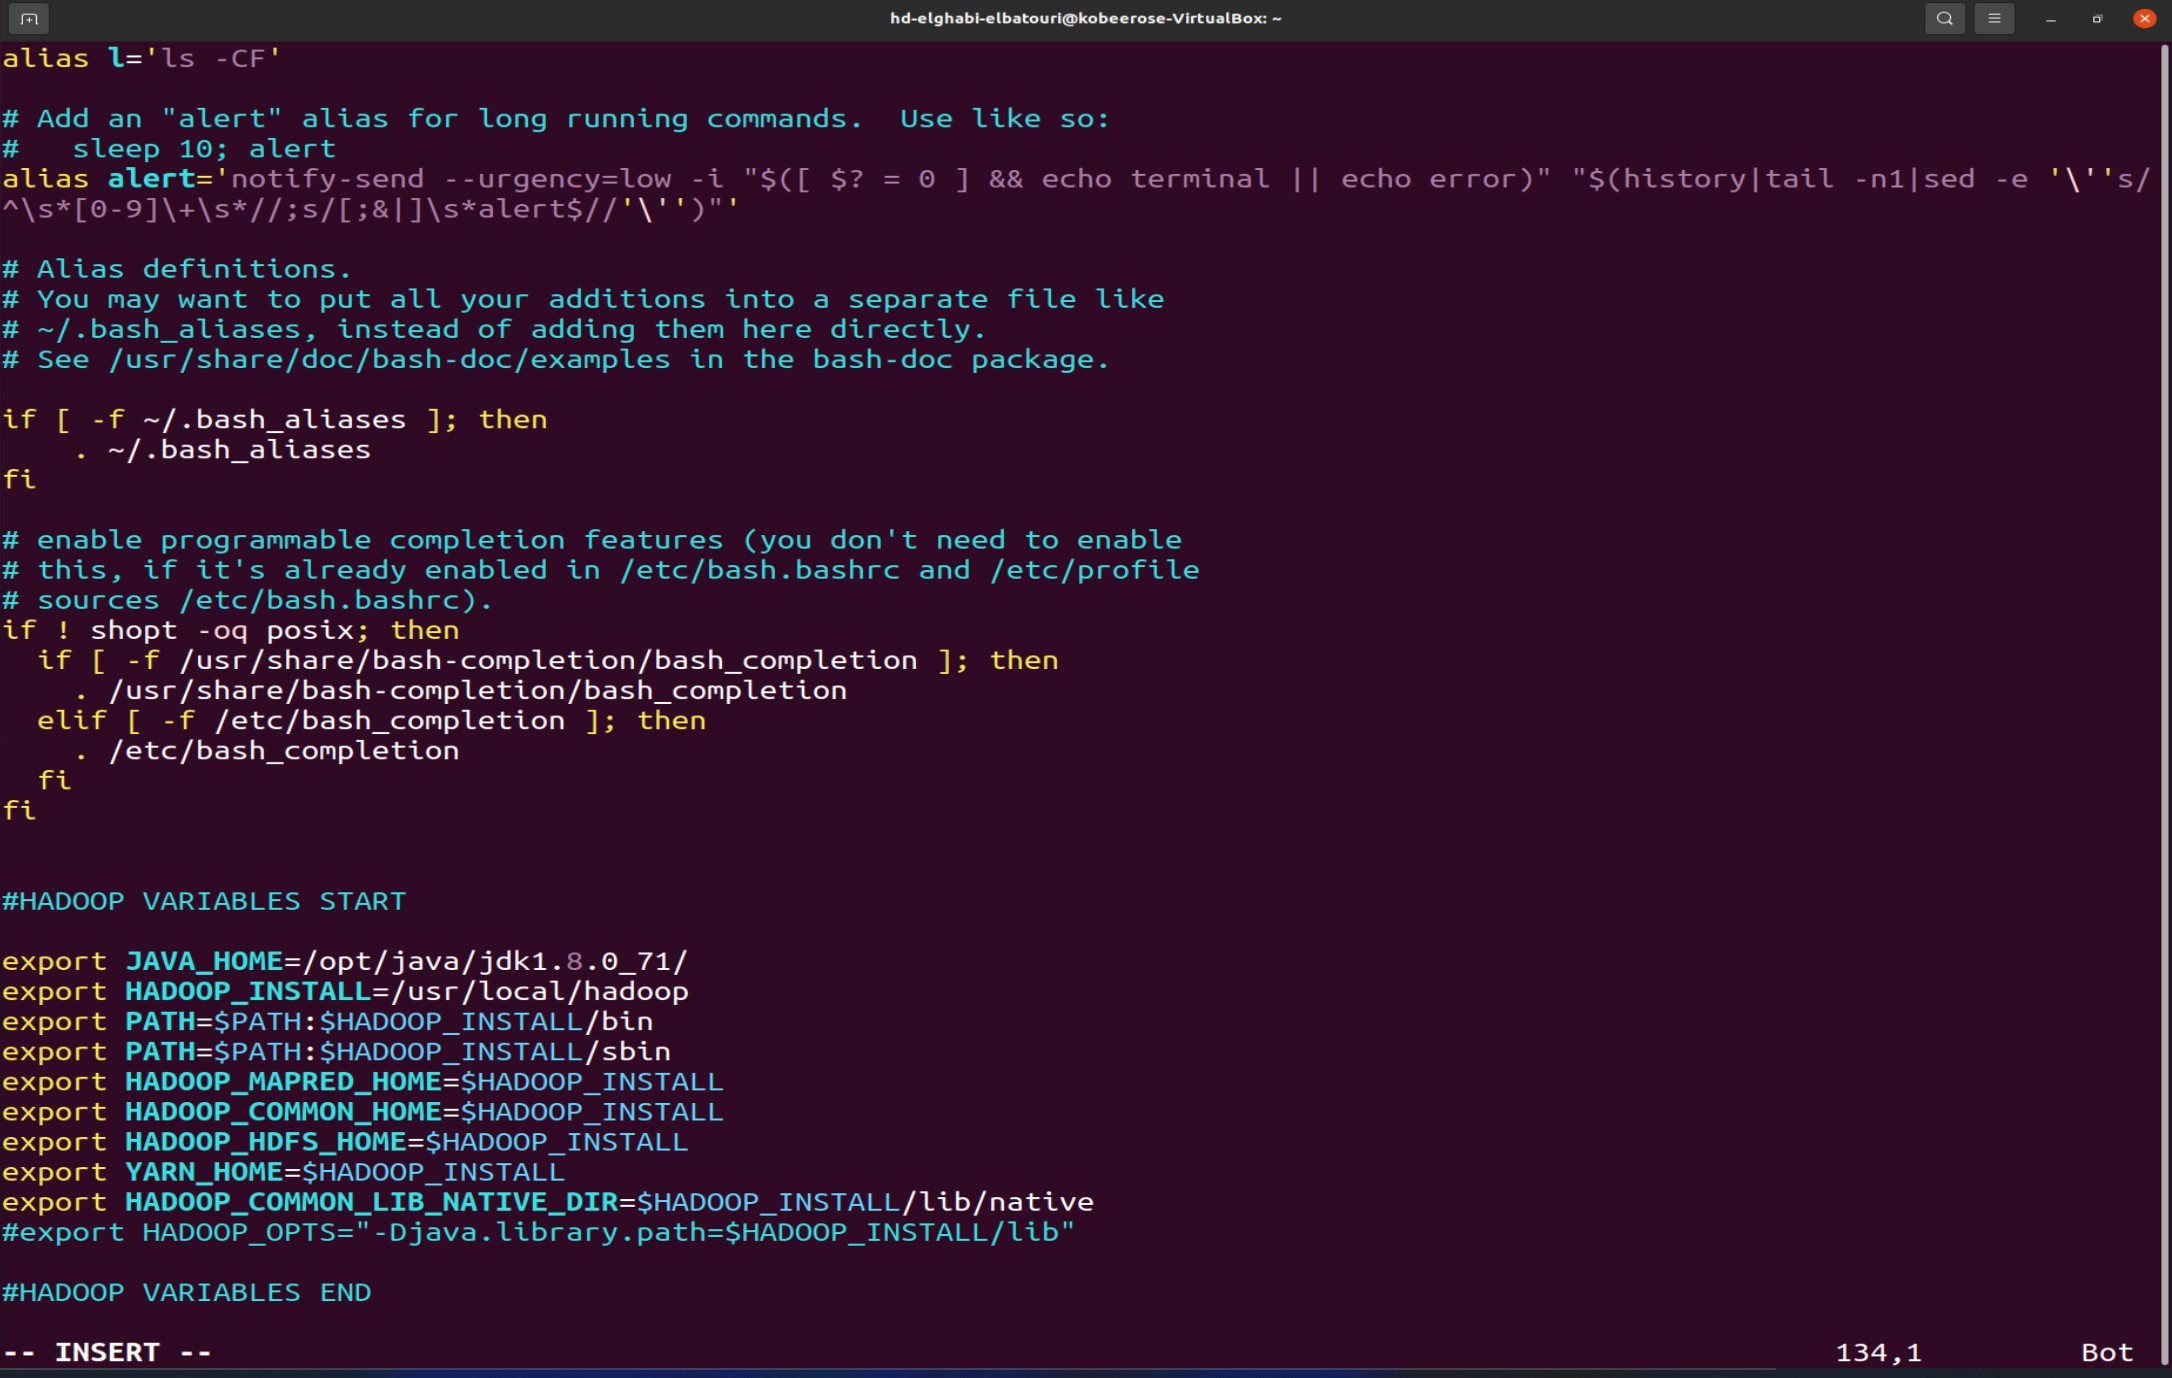
\includegraphics[width=1\linewidth]{Big_Data/Hadoop/Apache Hadoop Installation/Modifying .bashrc file} 
\end{center} 
\caption{Modifying .bashrc file} 
\end{figure} 
\FloatBarrier

\par Editing Hadoop Configuration Files: core-site.xml, hdfs-site.xml, mapred-site.xml, yarn-site.xml then Formatting of the Namenode. 
\\
\begin{figure}[!htb] 
\begin{center} 
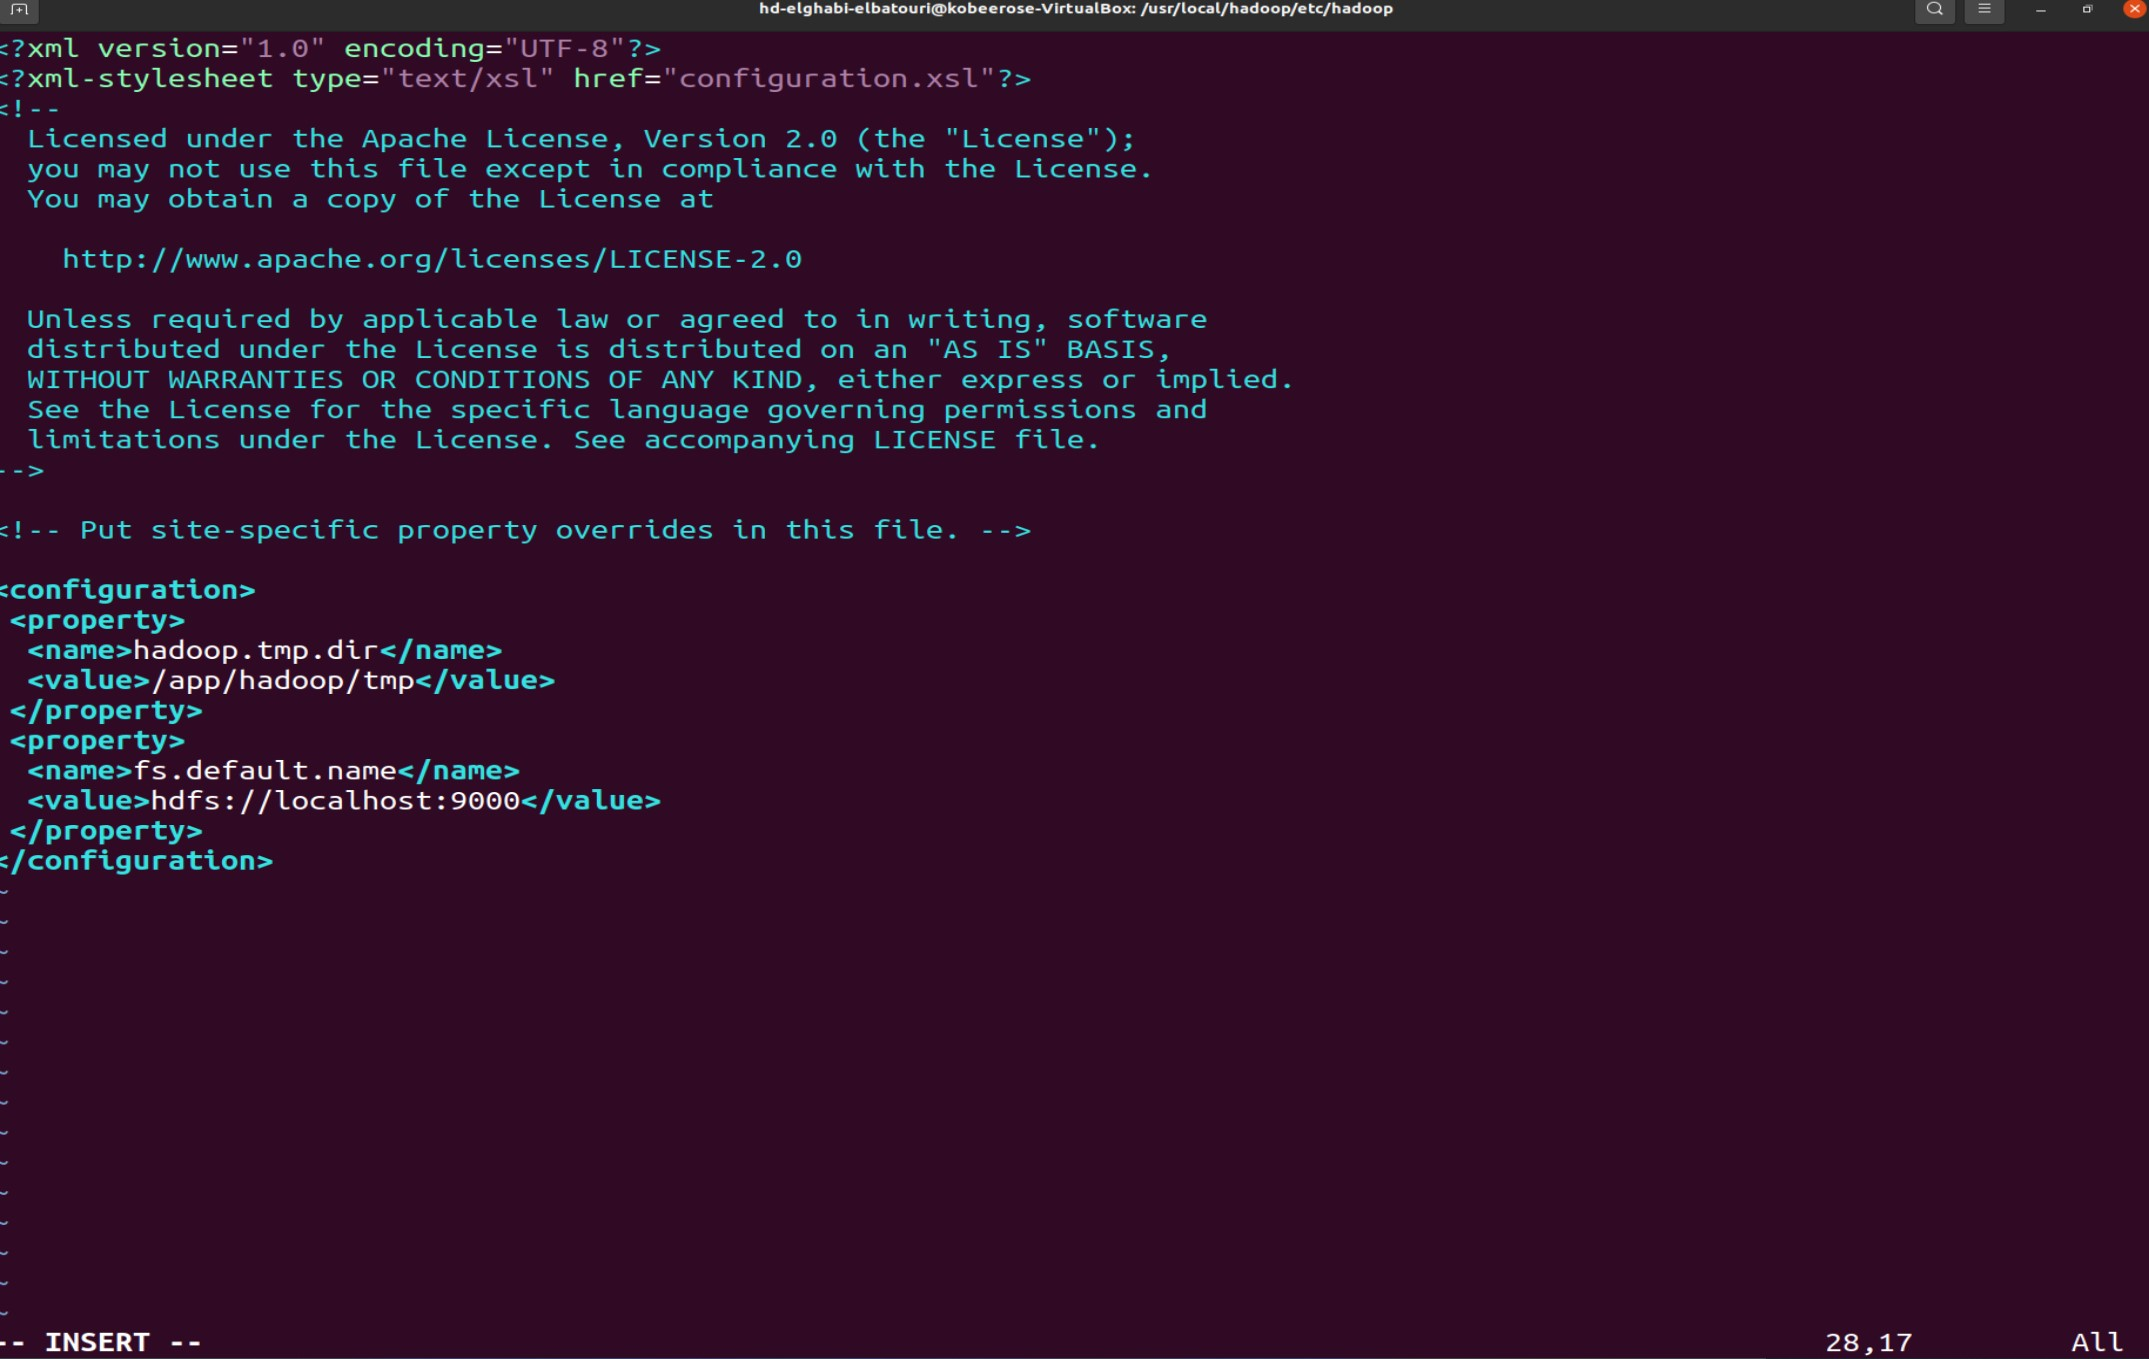
\includegraphics[width=1\linewidth]{Big_Data/Hadoop/Apache Hadoop Installation/core-site.xml config} 
\end{center} 
\caption{core-site.xml config} 
\end{figure} 
\FloatBarrier
\begin{figure}[!htb] 
\begin{center} 
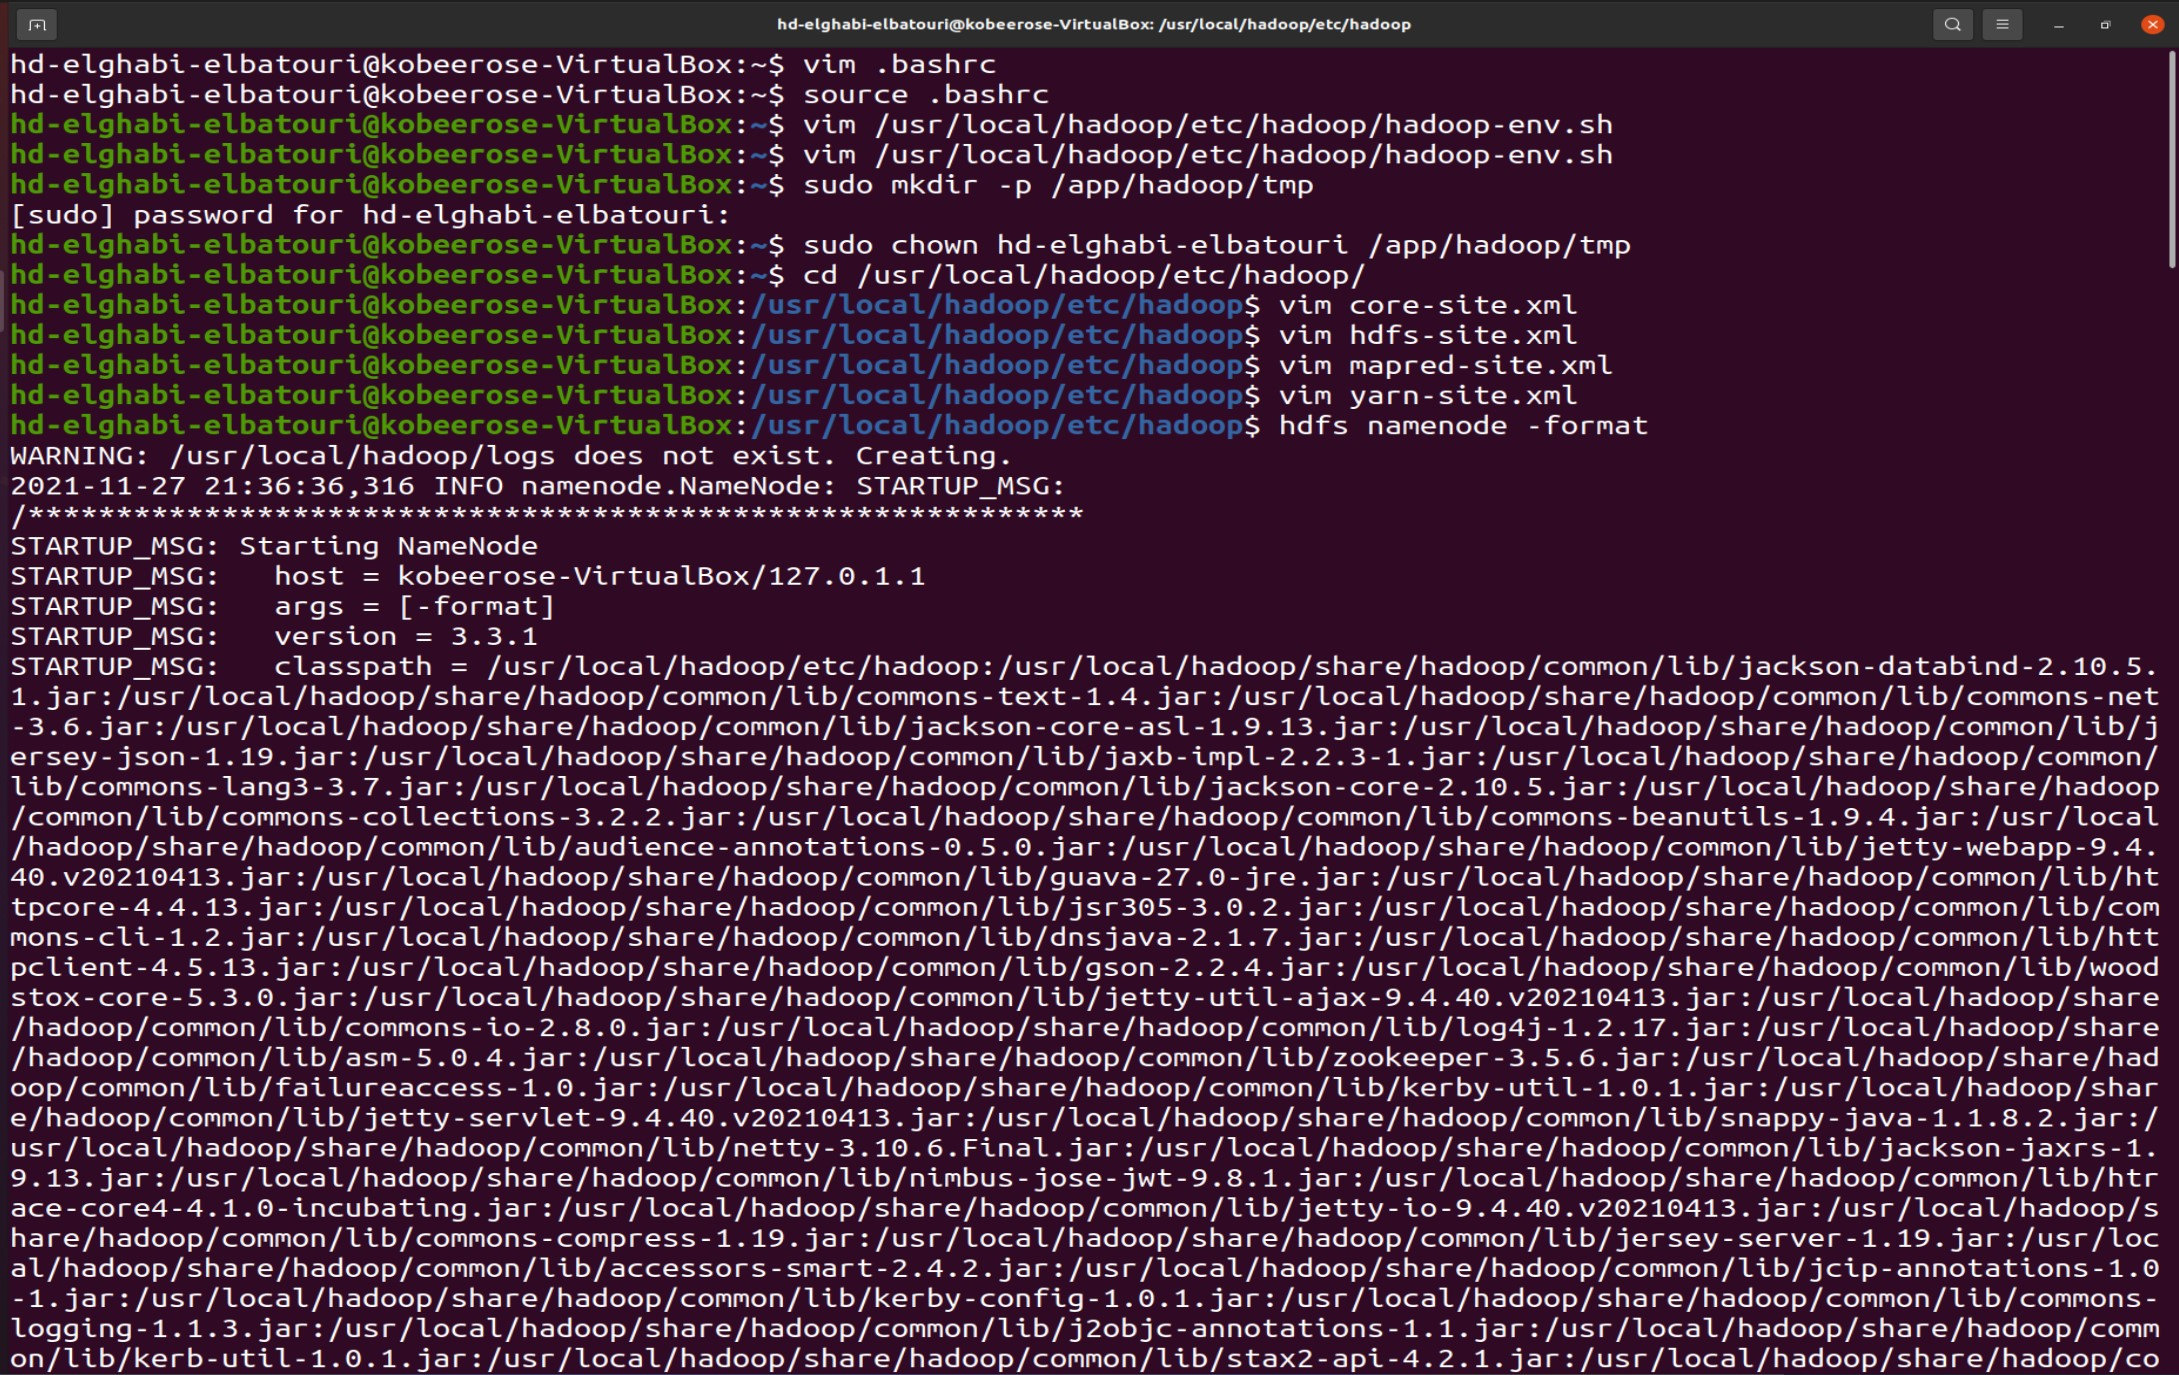
\includegraphics[width=1\linewidth]{Big_Data/Hadoop/Apache Hadoop Installation/Hadoop files configuration} 
\end{center} 
\caption{Hadoop files configuration} 
\end{figure} 
\FloatBarrier

\par Now it's time to start the newly installed single node cluster. 
\\
\begin{figure}[!htb] 
\begin{center} 
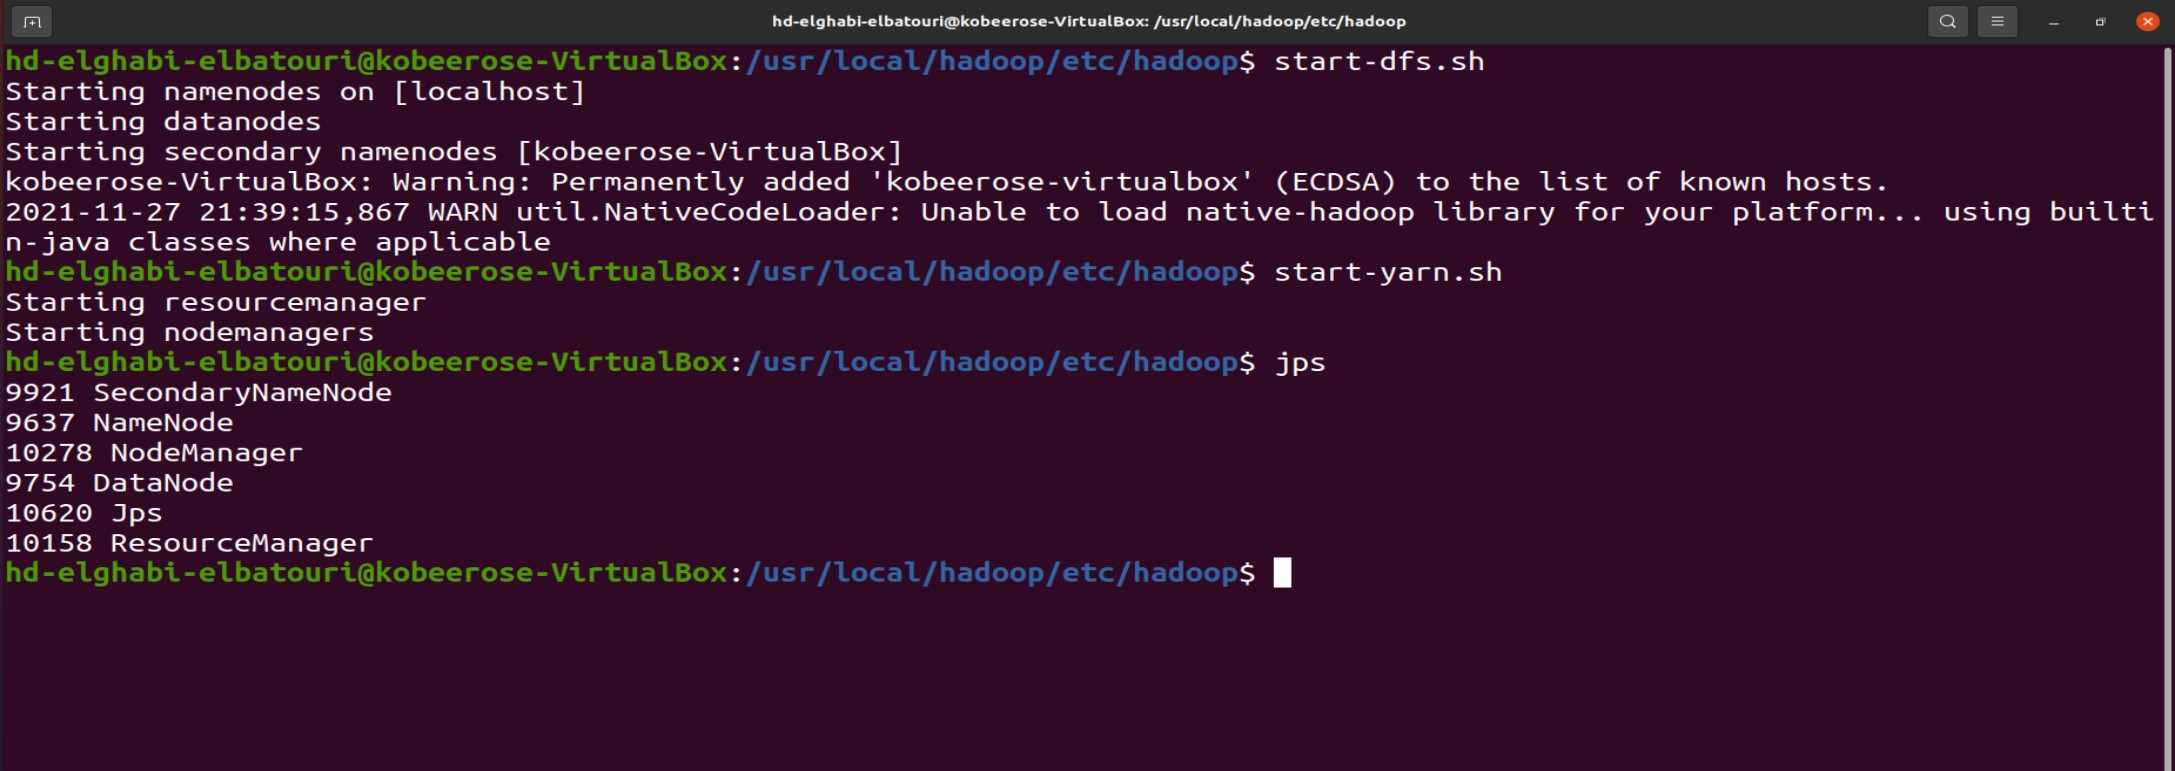
\includegraphics[width=1\linewidth]{Big_Data/Hadoop/Apache Hadoop Installation/Starting 1node Cluster} 
\end{center} 
\caption{Starting 1node Cluster} 
\end{figure} 
\FloatBarrier

\par Access Hadoop's graphical interfaces via the browser.
\\
\begin{figure}[!htb] 
\begin{center} 
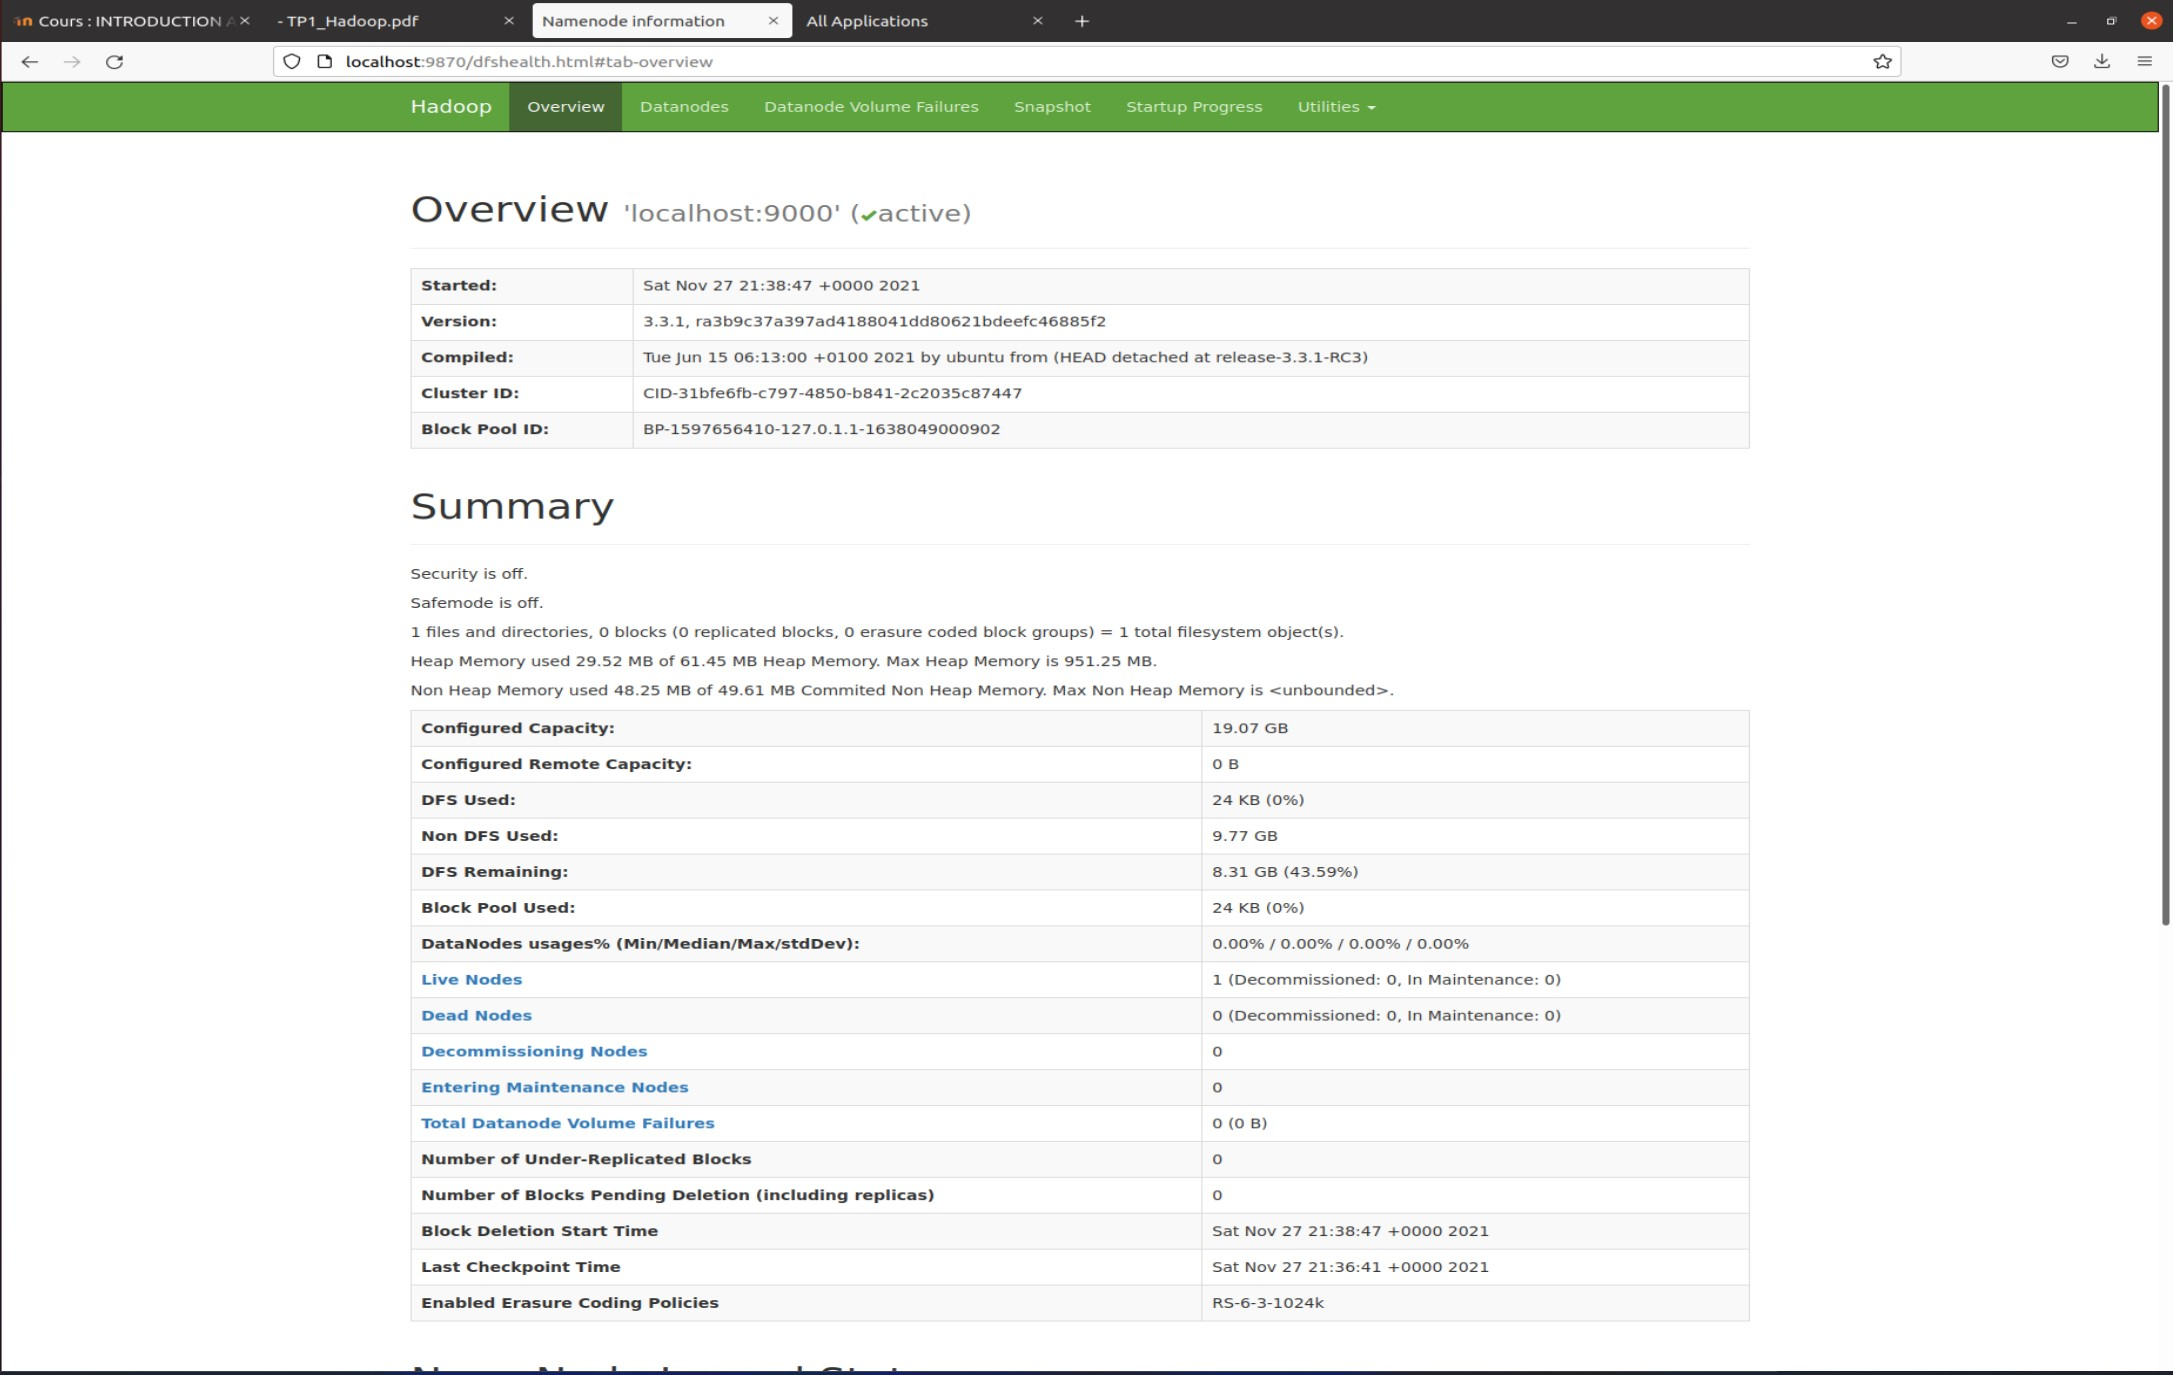
\includegraphics[width=1\linewidth]{Big_Data/Hadoop/Apache Hadoop Installation/Hadoop interface on port 9870} 
\end{center} 
\caption{Hadoop interface on port 9870} 
\end{figure} 
\FloatBarrier
\\
\begin{figure}[!htb] 
\begin{center} 
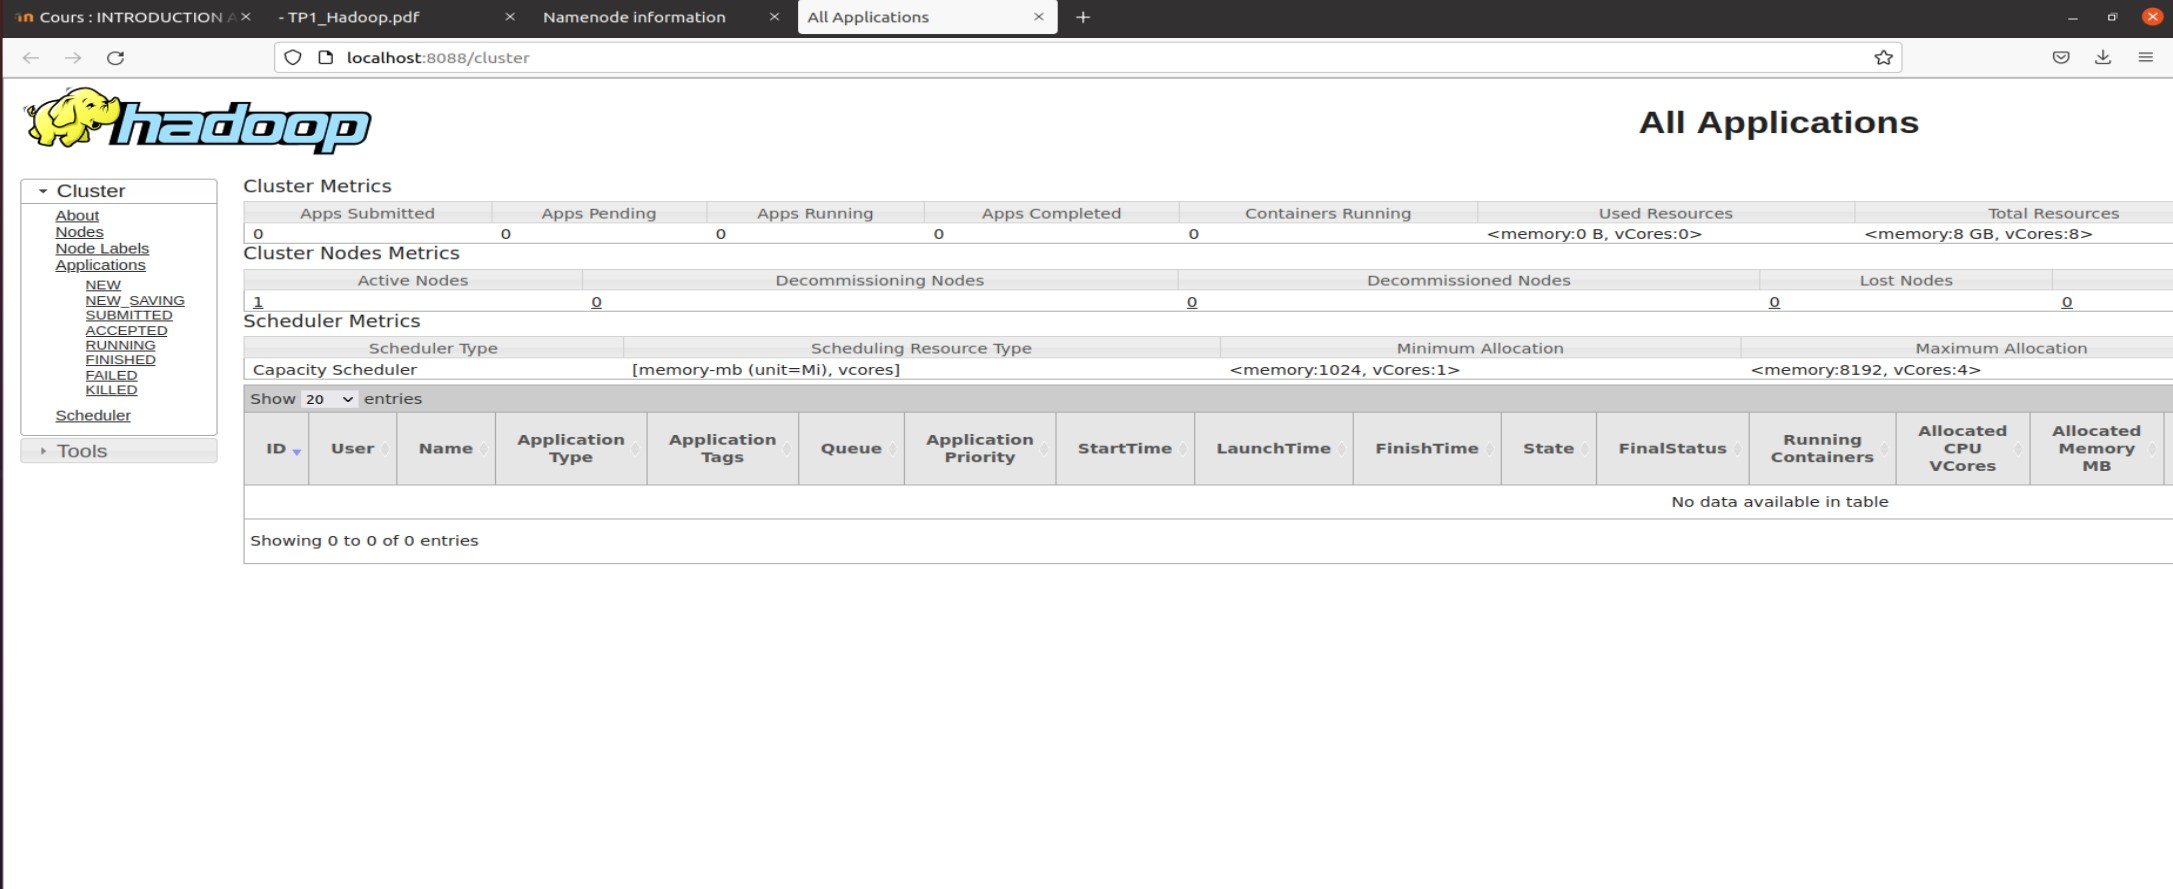
\includegraphics[width=1\linewidth]{Big_Data/Hadoop/Apache Hadoop Installation/ResourceManager Interface} 
\end{center} 
\caption{ResourceManager Interface} 
\end{figure} 
\FloatBarrier




\end{spacing}